\documentclass[journal]{vgtc}                % final (journal style)
%\documentclass[review,journal]{vgtc}         % review (journal style)
%\documentclass[widereview]{vgtc}             % wide-spaced review
%\documentclass[preprint,journal]{vgtc}       % preprint (journal style)

%% Uncomment one of the lines above depending on where your paper is
%% in the conference process. ``review'' and ``widereview'' are for review
%% submission, ``preprint'' is for pre-publication, and the final version
%% doesn't use a specific qualifier.

%% Please use one of the ``review'' options in combination with the
%% assigned online id (see below) ONLY if your paper uses a double blind
%% review process. Some conferences, like IEEE Vis and InfoVis, have NOT
%% in the past.

%% Please note that the use of figures other than the optional teaser is not permitted on the first page
%% of the journal version.  Figures should begin on the second page and be
%% in CMYK or Grey scale format, otherwise, colour shifting may occur
%% during the printing process.  Papers submitted with figures other than the optional teaser on the
%% first page will be refused. Also, the teaser figure should only have the
%% width of the abstract as the template enforces it.

%% These few lines make a distinction between latex and pdflatex calls and they
%% bring in essential packages for graphics and font handling.
%% Note that due to the \DeclareGraphicsExtensions{} call it is no longer necessary
%% to provide the the path and extension of a graphics file:
%% 
\includegraphics{diamondrule} is completely sufficient.
%%
\ifpdf%                                % if we use pdflatex
  \pdfoutput=1\relax                   % create PDFs from pdfLaTeX
  \pdfcompresslevel=9                  % PDF Compression
  \pdfoptionpdfminorversion=7          % create PDF 1.7
  \ExecuteOptions{pdftex}
  \usepackage{graphicx}                % allow us to embed graphics
                                % files
  \DeclareGraphicsExtensions{.pdf,.png,.jpg,.jpeg} % for pdflatex we expect .pdf, .png, or .jpg files
\else%                                 % else we use pure latex
  \ExecuteOptions{dvips}
  \usepackage{graphicx}                % allow us to embed graphics files
  \DeclareGraphicsExtensions{.eps}     % for pure latex we expect eps files
\fi%

%% it is recomended to use ``\autoref{sec:bla}'' instead of ``Fig.~\ref{sec:bla}''
\graphicspath{{figures/}{pictures/}{images/}{./}} % where to search for the images

\usepackage{microtype}                 % use micro-typography (slightly more compact, better to read)
\PassOptionsToPackage{warn}{textcomp}  % to address font issues with \textrightarrow
\usepackage{textcomp}                  % use better special symbols
\usepackage{mathptmx}                  % use matching math font
\usepackage{times}                     % we use Times as the main font
\renewcommand*\ttdefault{txtt}         % a nicer typewriter font
\usepackage{cite}                      % needed to automatically sort the references
\usepackage{tabu}                      % only used for the table example
\usepackage{booktabs}                  % only used for the table example
\usepackage[]{algorithm2e}
\usepackage{color}
\usepackage{amsmath}
\usepackage{cleveref}
%% We encourage the use of mathptmx for consistent usage of times font
%% throughout the proceedings. However, if you encounter conflicts
%% with other math-related packages, you may want to disable it.

%% In preprint mode you may define your own headline.
%\preprinttext{To appear in IEEE Transactions on Visualization and Computer Graphics.}

%% If you are submitting a paper to a conference for review with a double
%% blind reviewing process, please replace the value ``0'' below with your
%% OnlineID. Otherwise, you may safely leave it at ``0''.
\onlineid{0}

%% declare the category of your paper, only shown in review mode
\vgtccategory{Research}
%% please declare the paper type of your paper to help reviewers, only shown in review mode
%% choices:
%% * algorithm/technique
%% * application/design study
%% * evaluation
%% * system
%% * theory/model
\vgtcpapertype{please specify}

%% Paper title.
\title{A Study of Task-dependent, Precision-adaptive Data Streams for Scientific Analytics}

%% This is how authors are specified in the journal style

%% indicate IEEE Member or Student Member in form indicated below
\author{Roy G. Biv, Ed Grimley, \textit{Member, IEEE}, and Martha Stewart}
\authorfooter{
%% insert punctuation at end of each item
\item
 Roy G. Biv is with Starbucks Research. E-mail: roy.g.biv@aol.com.
\item
 Ed Grimley is with Grimley Widgets, Inc.. E-mail: ed.grimley@aol.com.
\item
 Martha Stewart is with Martha Stewart Enterprises at Microsoft
 Research. E-mail: martha.stewart@marthastewart.com.
}

%other entries to be set up for journal
\shortauthortitle{Biv \MakeLowercase{\textit{et al.}}: Global Illumination for Fun and Profit}
%\shortauthortitle{Firstauthor \MakeLowercase{\textit{et al.}}: Paper Title}

%% Abstract section.
\abstract{Performing scientific analysis on petabytes of data commonly found nowadays is an onerous task
due to the prohibitive cost of data transfer. Currently this issue is alleviated by working with
reduced-resolution or reduced-precision data. This paper brings together techniques that reduce data
in resolution, precision, and both, into a common framework in which they can be studied and
compared. The error patterns of these techniques are compared with regards to fundamental metrics, namely L2 norm,
first and second derivatives, histograms, and isocontours. We also compute and study
metric-dependent streams which serve as empirical bounds on the limit to which
reduction can happen, given an error tolerance for the analysis task at hand. Finally, based on the
observed characteristics of those streams, we propose practical heuristics to minimize the amount of
data needed to perform a given analysis task. The insights and heuristics presented here can be
leveraged to implement data-optimal representations and querying systems to facilitate interactive
exploration as well as cursory analysis of enormous data.%
} % end of abstract

%% Keywords that describe your work. Will show as 'Index Terms' in journal
%% please capitalize first letter and insert punctuation after last keyword
\keywords{Radiosity, global illumination, constant time}

%% ACM Computing Classification System (CCS). 
%% See <http://www.acm.org/class/1998/> for details.
%% The ``\CCScat'' command takes four arguments.

\CCScatlist{ % not used in journal version
 \CCScat{K.6.1}{Management of Computing and Information Systems}%
{Project and People Management}{Life Cycle};
 \CCScat{K.7.m}{The Computing Profession}{Miscellaneous}{Ethics}
}

%% Uncomment below to include a teaser figure.
%\teaser{
%  \centering
%  \includegraphics[width=\linewidth]{CypressView}
%  \caption{In the Clouds: Vancouver from Cypress Mountain. Note that the teaser may not be wider than the abstract block.}
%	\label{fig:teaser}
%}

%% Uncomment below to disable the manuscript note
%\renewcommand{\manuscriptnotetxt}{}


\newcommand{\norm}[1]{\left\lVert#1\right\rVert}
\newcommand{\notetext}[1]{%
  \raggedright\tiny\sffamily\bfseries{#1}%
}
\newcommand{\note}[1]{%
  \ifinner%
    \smash{%
      \raggedright%
      \hspace*{\textwidth}%
      \hspace*{\marginparsep}%
      \parbox[t]{\marginparwidth}{\notetext{#1}}%
    }%
    \\[-0.5\bs]%
  \else%
    \marginpar{\notetext{#1}}%
  \fi%
}

\newcommand{\ptb}[1]{{\textcolor{red}{(PTB: #1)}}}
\newcommand{\pavol}[1]{{\textcolor{cyan}{(Pavol: #1)}}}
\newcommand{\hb}[1]{{\textcolor{blue}{(HB: #1)}}}


%% Copyright space is enabled by default as required by guidelines.
%% It is disabled by the 'review' option or via the following command:
% \nocopyrightspace

\vgtcinsertpkg
\usepackage{subcaption}

%%%%%%%%%%%%%%%%%%%%%%%%%%%%%%%%%%%%%%%%%%%%%%%%%%%%%%%%%%%%%%%%
%%%%%%%%%%%%%%%%%%%%%% START OF THE PAPER %%%%%%%%%%%%%%%%%%%%%%
%%%%%%%%%%%%%%%%%%%%%%%%%%%%%%%%%%%%%%%%%%%%%%%%%%%%%%%%%%%%%%%%%

\begin{document}

%% The ``\maketitle'' command must be the first command after the
%% ``\begin{document}'' command. It prepares and prints the title block.

%% the only exception to this rule is the \firstsection command
\firstsection{Introduction}

\maketitle

As the gap between the available compute power and the cost of data movement increases, data
transfer, whether from cache, main memory, or from disk, becomes a major bottleneck in many
workflows. However, it has been shown that not every bit of data is always necessary to answer
scientific questions with required accuracy. In particular, for techniques at the end of scientific
workflows, such as visualization and data analysis, lower fidelity representations of the data often
provide adequate approximations~\cite{woodring2011,covra2012,compression_sim2013}, and even during
simulation some loss in precision is often
acceptable~\cite{compression_sim2013,doi:10.1177/1094342018762036}. As a result, several different
techniques have been proposed to reduce the size of data. 

Broadly, these techniques can be classified into (i) reducing the data resolution, e.g., the number
of data points stored, and (ii) reducing the precision of each data point. Examples of the former
kind of approaches are subsampling~\cite{idx2001}, adaptive mesh refinement~\cite{amr1989}, octrees
and other tree structures~\cite{hierarchical1984}, and wavelets~\cite{woodring2011}, and those of
the latter are various forms of
compression~\cite{fpzip,isabela,zfp2014,sz,vq1992,compression_domain2003,sqe}. Traditionally,
multiresolution structures have been used to accelerate dynamic queries, e.g., in
rendering~\cite{multires_octree1999}, since discarding data points based on the viewpoint or data
complexity can result in significant speed-up. Compression based on quantization, on the other hand,
is more common when storing data, where in the absence of other information, treating each sample as
equally important is the null hypothesis. However, in many situations, a combination of both
resolution and precision reduction could be appropriate. For example, high spatial resolution may be
needed to resolve the topology of an isosurface, yet the corresponding data samples may be usable at
less than full precision to adequately approximate the geometry. Conversely, accumulating accurate
statistics may require high-precision values, yet a lower resolution subset of data points may be
sufficient for the task. 

In general, different levels of adaptivity in combinations of resolution and precision may be
suitable for different types of analysis and visualization tasks, and for many, these requirements
will be data dependent. Consequently, a globally optimal data organization may not exist. Instead,
we consider a progressive setting in which some initial data is loaded and processed, and new data
is requested selectively based on the requirement of the current task as well as the characteristics
of the data already loaded. The result is a stream of bits ordered such that the error is minimized,
considering the task at hand. However, although intuitively there are almost certainly advantages in
considering both resolution and precision in the ordering, it is unclear how much the error could be
reduced for a given data budget or how little data could be used to achieve the same error.
Furthermore, optimal data-dependent orderings may be especially impractical since they assume
perfect knowledge of the data. It is therefore important to understand which of these potential
gains are realizable. This paper aims to answer these important questions about the suitable bit
orderings through extensive, empirical experiments. In particular, this paper presents:

\begin{itemize}\dense
%
\item a framework that allows systematic studies of the resolution-versus-precision tradeoffs for
common data analysis and visualization tasks. The core idea is to represent various data reduction
techniques as bit streams that improve data quality in either resolution or precision in each step
(\Cref{sec:terminologies}). We can thus compare these techniques fairly, by comparing the
corresponding data streams.
%  
\item empirical evidence that jointly optimizing resolution and precision can provide significant
improvements on the results of analysis tasks over adjusting either independently. 
We present a diverse collection of data sets and data analysis tasks, and also show how
different types of data analysis might require substantially different data streams for optimal
results.
%
\item a greedy approach that gives estimations for lower bounds of error for various analysis tasks.
In addition, we also identify practical streams that closely approximate these bounds for each task
(\Cref{sec:rmse-optimized}, \Cref{sec:derivatives}, \Cref{sec:histogram}, and
\Cref{sec:isocontour}), using a novel concept called \emph{stream signature}
(\Cref{sec:stream-signature}), which is a small matrix that captures the essence of how a bit stream
navigates the precision-versus-resolution space.
\end{itemize}


%%% Local Variables:
%%% mode: latex
%%% TeX-master: "template"
%%% End:

\section{Related work}

\para{Tree-based multiresolution hierarchies.}
Techniques that reduce data in resolution typically build a tree-shape hierarchy over the data. A
very common scheme to generate such a hierarchy is to construct low-resolution copies of the data
from higher resolution ones through filtering or subsampling. Examples include Gaussian and
Laplacian pyramids~\cite{laplacian-pyramid},
mipmaps~\cite{multires_octree1999,interactive-exploration-ct-scans}. Often, the data is stored in
blocks on each resolution level. To save bandwidth, low-resolution blocks can be streamed during
rendering, if the points being queried project to less than a pixel on screen. However, these
methods increase storage requirements and potentially expensive pre-processing, making them
unsuitable for very large data.

Recent multi-resolution techniques save storage by adapting to the data in such a way that different
regions of the data are stored in different resolutions and depending on how ``homogeneous'' is the region.
Fast-varying regions are stored at higher resolution. A very popular approach is sparse voxel
octrees (SVO), pioneered by Crassin \etal~\cite{gigavoxels} and Gobbetti \etal~\cite{Gobbetti2008},
and variations of which are found in~\cite{Fogal-2013-RayGuided,visualization-driven}. Sparsity
comes from the fact that smooth-varying regions are stored at coarser octree levels, which
significantly reduces storage. During rendering, blocks of samples are streamed from an appropriate
resolution, determined by how far the queried samples are from the eye/camera. Beyer
\etal~\cite{large‐scale-volume} give a comprehensive overview of state-of-the-art GPU-based
out-of-core ray-casting techniques.

Beside octrees, other trees such as B+ tree~\cite{vdb2013} and
kd-tree~\cite{fogal-kdtree,in-situ-sampling-particle} can also be used to build a sparse hierarchy.
Alternatively, space-filling curves such as the hierarhical Z curve~\cite{idx2001} or the Hillbert
curve~\cite{mloc} can be used to reorder data samples to form a hierarchy without any filtering
steps or redundant samples, as low-resolution levels are constructed via subsampling. Unfortunately,
subsampling can introduce aliasing.

%\paragraph{\textbf{Transform-based multiresolution hierarchies}}
\para{Transform-based multiresolution hierarchies.}
Other multiresolution approaches reduce data by transform-based compression. For example,
COVRA~\cite{covra2012} constructs an octree of bricks, each of which is further subdivided \pavol{into?} blocks.
Compression is done by learning a sparse representation for the blocks in terms of prototype (basis)
blocks. Similarly, Fout\etal~\cite{hw_dvr2007} transform each block in the volume using the KLT
transform, which produces several classes of partitions (each can be thought of as one resolution
level). They compress the transform coefficients using vector quantization~\cite{vq1992} by
constructing one codebook for each paritition class. Schneider~\etal~\cite{compression_domain2003}
also use vector quantization on transform coefficients, but with a simple Haar-like transform that
separates each block of $2^3$ voxels into one average and seven difference coefficients.

Analogous to the KLT transform in 2D, the Tucker decomposition~\cite{tensor_dvr2015} in
$n$-dimensional space decomposes the input data (stored as a tensor) into $n$ matrices of basis
vectors and one core tensor. Reduction in storage and in transmission bandwidth comes from the fact
that the basis matrices can be downsampled (resulting in a lower resolution representation) and the
core tensor can be rank-truncated (resulting in coarse-scale representations of
features)~\cite{tamresh,tucker-thresholding,multiscale-tensor}. Furthermore, elements in the basis
matrices and the core tensor can be thresholded~\cite{tucker-thresholding} or
quantized~\cite{tamresh,multiscale-tensor}. Tensor decomposition can work for higher dimensional
data and can achieve very high compression ratios. However, the transform step is costly due to it
being data-dependent.

%\paragraph{\textbf{Wavelets}}
\para{Wavelets.}
Transforms that use fixed bases avoid such high computation cost at the expense of slightly less
effective compression. Perhaps the most popular transform that uses a fixed basis is the (discrete)
wavelet transform (DWT). The DWT constructs a hierarchy of resolution levels via low and high
bandpass filters. The transform is recursively applied to the lower resolution band, resulting in a
hierarchy of ``details'' at varying resolution. One benefit of wavelets over redundant
representations such as Laplacian pyramids is that the wavelet transform is merely a change of basis
that like reordering techniques does not increase the data size. Another benefit over adaptive
refinement meshes and other tree-like techniques is that the wavelet basis functions are defined
everywhere in space, requiring no special interpolation rules when given some arbitrary subset of
wavelet coefficients and basis functions. One disadvantage of the wavelet transform is the random
access cost, which is not constant time. However, there has been work to develop acceleration
structures to speed up local queries~\cite{weiss}.

Beside offering a multiresolution decomposition, enabling data streaming with level-of-detail
support, wavelets also offer ample opportunities for compression. As the magnitude of wavelet
coefficients decays rapidly for a typical volume [CITE], they are especially amenable to thresholding
or entropy compression. In the context of storing and visualizing scientific data, wavelets (with
compression) are used in a wide variety of
systems~(\cite{multires_toolkit2003,vapor2007,woodring2011}) and applications (volume rendering
with
level-of-detail~\cite{wavelet-compression-interactive-vis,multires-framework,rapid-compression-volume,interactive-rendering-large-volume,multires-volume-rendering},
turbulence visualization~\cite{treib}, particle visualization~\cite{sph-octree}).

Most wavelet-based techniques employ tiling of wavelet coefficients in individual subands to
facilitate random access and spatial adaptivity in resolution. For example, the VAPOR
toolkit~\cite{vapor2007} incorporates a multiresolution file format based on a wavelets to allow
data analysis on commodity hardware by storing individual tiles in separate files to allow loading
of the region of interest. However, like most multiresolution work, only the resolution control is
leveraged. The precision axis, which can potentially further reduce data transfer, is left
unexplored.

%\paragraph{\textbf{Wavelet coders}}
\para{Wavelet coders.}
Most work that explores the precision axis comes from state-of-the-art coders for wavelet
coefficients in image compression. Wavelet coefficients in corresponding regions across subbands can
be thought of as belonging to a ``tree'', with the root being a single coefficient at the lowest
subband. Thee emmbedded zerotrees (EZW) coder exploits the property that in such trees, ``parent''
coefficients are often larger in magnitude than ``child'' coefficients. It locates trees of wavelet
coefficients that are insignificant with regard to (i.e., less than in magnitude) a threshold. Such
a tree is encoded with one single symbol, resulting in significant compression. The threshold is
typically set at each bit plane, starting from the most significant one. In this way, the data can
be progressively refined in precision during decompression. The SPIHT coder~\cite{spiht1996}
improves on EZW by locating more general types of zero trees~\cite{quantifying-coding-performance}.
SPECK~\cite{speck2004} extends SPIHT to exploit also spatial correlations among nearby coefficients
on the same subband.

%\paragraph{\textbf{Floating-point compression}}
\para{Floating-point compression.}
\newcommand{\zfp}{\textsc{zfp}\xspace}
The \zfp compression scheme~\cite{zfp2014} also encodes transform coefficients by bit plane, in
order of decreasing significance. \zfp partitions the domain---a structured grid---into small (e.g.,
$4 \times 4 \times 4$) independent blocks and thus allows for localized decompression. Moreover,
\zfp supports fixed-rate compression that facilitates random access to the data. Its fast transform
and caching of decompressed data allows it to achieve not only high throughput decompression, but
also fast inline compression. Extensions of \zfp allow it to vary either the bit rate or precision
spatially over the domain, albeit at fixed resolution~\cite{zfp-arc}. Other notable compression
schemes for scientific data include scalar quantization encoding (SQE)~\cite{sqe},
ISABELA~\cite{isabela}, SZ~\cite{sz}, and FPZIP~\cite{fpzip}. The latter three employ prediction and
compress the residuals. ISABELA and SZ perform residual scalar quantization, whereas FPZIP truncates
floats, which can be seen as nonuniform scalar quantization. Similar to FPZIP, the precision-based
level of details (PLoD) scheme proposed in MLOC~\cite{mloc} also truncates floats by dividing a
double-precision number into seven parts, of which the first part contains the first two bytes, and
each of the other six parts contains one byte for additional precision. MLOC includes a
multiresolution scheme based on Hillbert curves, but this scheme (based on resolution) and the PLoD
scheme (based on precision) are exclusive.

%\paragraph{\textbf{Mixing resolution and precision}}
\para{Mixing resolution and precision.}
Schemes that allow progressive data access in both resolution and precision include
SBHP~\cite{sbhp2000} and JPEG2000~\cite{jpeg2000}. Both partition each subband into blocks and code
each block independently, in bit plane order. By interleaving compressed bits across blocks, one can
construct a purely resolution-progressive or a purely precision-progressive stream, or anything in
between. Outside image compression, JPEG2000 has found use in the compression of scientific data. For
example, Woodring \etal~\cite{woodring2011} use JPEG2000 to store floating point data. Since most
JPEG2000 implementations are limited to integer data, the authors apply uniform scalar quantization
to convert floating point data to integer form. Even though JPEG2000 supports varying both
resolution and precision, the authors do not explore this capability but focus only on setting bit
rate. In general, although there exist mechanisms that simultaneously leverage both axes of data
reduction, especially for the purpose of scientific data analysis, they have not been
well-studied.

%\paragraph{\textbf{Error quantification}}
\para{Error quantification.}
Several works have aimed at quantifying the error incurred by data reduction, by
compression or otherwise, for the results of analysis tasks. Baker
\etal~\cite{evaluating-compression-climate} evaluate several compressors (FPZIP~\cite{fpzip},
APAX~\cite{apax}, ISABELA~\cite{isabela}) on ensembles of climate simulation data, using the
root-mean-square z-score (RMSZ) as the error metric. Laney \etal~\cite{compression_sim2013} study
the effects of lossy compression (using FPZIP and APEX) on the Miranda hydrodynamic simulation code,
using physics-based error metrics. Li \etal~\cite{evaluating-efficacy-wavelet} measure the error
incurred by wavelet compression on turbulent-flow data, using root-mean-square error of
radial-enstrophy profiles as the metric. Wang \etal~\cite{statistical-volume-quality} assess the
quality of distorted data using a combination of statistical metrics in the wavelet transform
domain. Etiene \etal have published a series of studies on verification of isosurfaces in
geometrical~\cite{verifiable-isosurface} and topological~\cite{topology-verification-isosurface}
terms, as well as verification of volume-rendered images~\cite{verifying-volume-rendering}. They
focus on order-of-accuracy and convergence analysis, where errors are introduced mostly through
discretization, not necessarily for the purpose of reducing data bandwidth. Finally, the Z-checker
framework~\cite{z-checker} consists of many independent metrics (which are called analysis
``kernels'') to evaluate data quality after lossy compression. The list includes min/max,
distribution, entropy, smoothness, power spectrum, principal component analysis, and
autocorrelation. In general, however, no studies have examined the
resolution-versus-precision tradeoffs, as well as the various orderings of bits in the context of
data analysis and visualization.

%by magnitude streams~\cite{image_compression1992}
% Transfer function adaptive decompression~\cite{tf_decompression2004}

Finally, for surveys of data reduction techniques in general, we refer the readers to the work of
Rodr\'{\i}guez \etal~\cite{state-of-the-art-compressed-volume} and Li \etal~\cite{li2018}.

\section{The advantages of combining resolution and precision}
\label{sec:motivation}

Traditional data reduction techniques work by either truncating the finest few resolution levels, or
truncating the last few low-ordered bits of every sample, but rarely both. In this section, our aim
is to show that significant gain can be achieved when one combines both dimensions, namely
resolution and precision, for data reduction. To do so, for each data set, we construct and compare
three different streams, which use different sorting criteria to sort the same set of chunks in
decreasing order of weights. We will use $W(c)$ to denote a sorting criteria, which is any function
that takes a chunk $c$ and returns its `'weight'' that determines its importance.

We compare the three streams by plotting an error curve for each, with regards to three error
metrics, namely root-mean-square error (Figure \ref{fig:motivation-rmse}), histogram error (Figure
\ref{fig:motivation-histogram}), and isocontour error (Figure \ref{fig:motivation-isocontour}). For
each metric, the function is reconstructed every time a new chunk is received from a stream, then
the relevant quantity (the function itself, its histogram, or an isocontour) is computed from the
reconstructed function, and compared against the same quantity computed from the original (lossless)
function. The definitions of histogram error and isocontour error are discussed in detail in Section
[REF] and Section [REF] respectively.

\begin{figure}[h]
  \centering
	\subcaptionbox{Boiler}
  {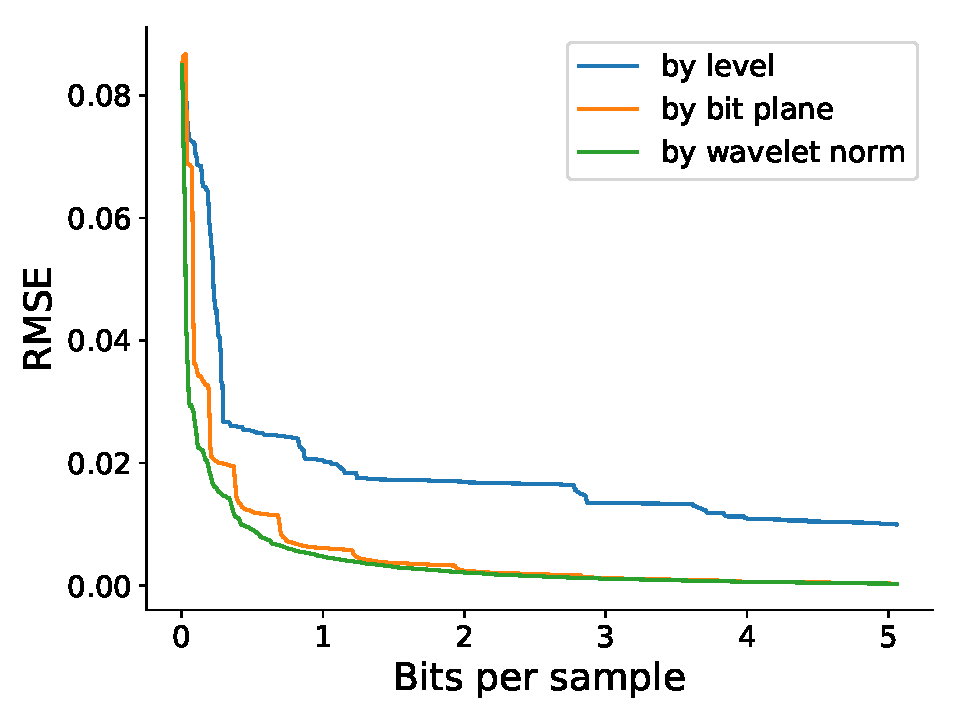
\includegraphics[width=0.48\linewidth]{img/motivation/motivation-psnr-boiler.pdf}}
	\subcaptionbox{Diffusivity}
 	{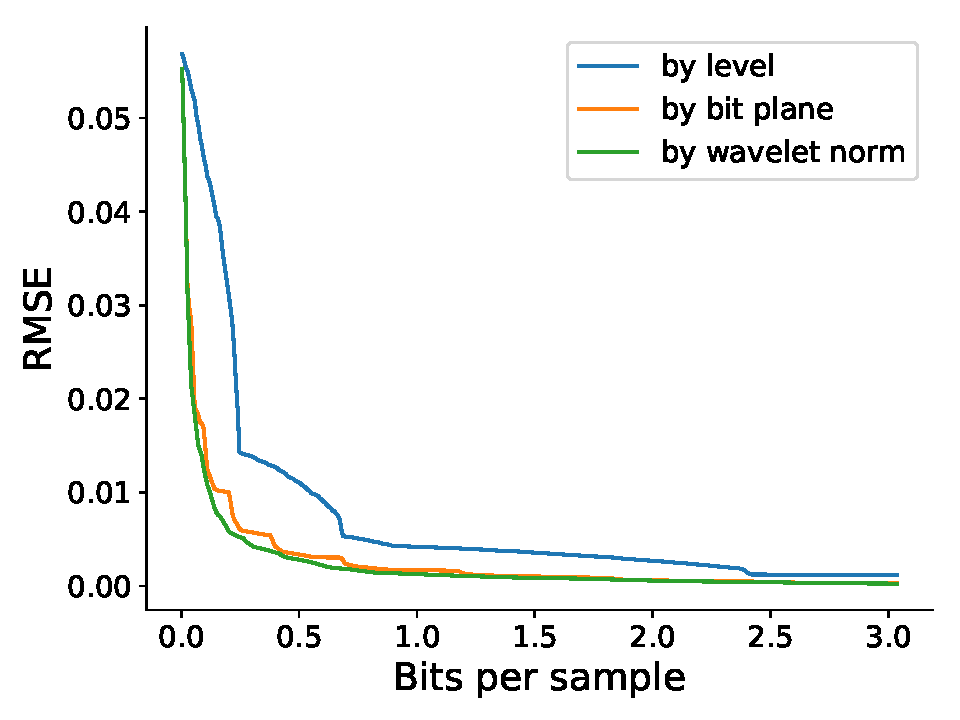
\includegraphics[width=0.48\linewidth]{img/motivation/motivation-psnr-diffusivity.pdf}}
	\subcaptionbox{Euler}
 	{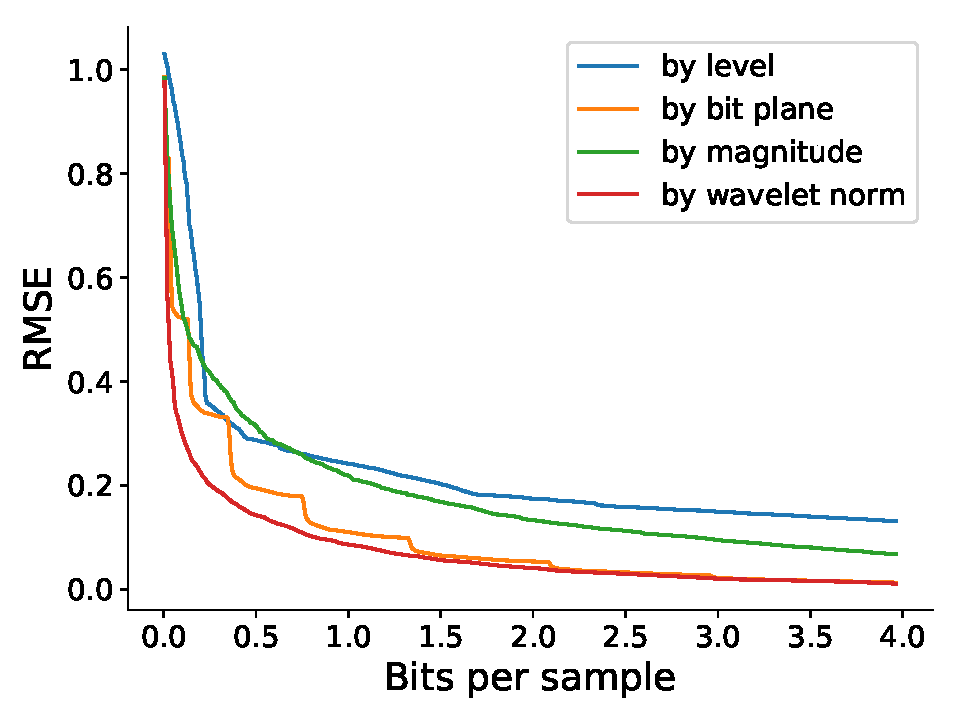
\includegraphics[width=0.48\linewidth]{img/motivation/motivation-psnr-plasma.pdf}}
	\subcaptionbox{Turbulence}
 	{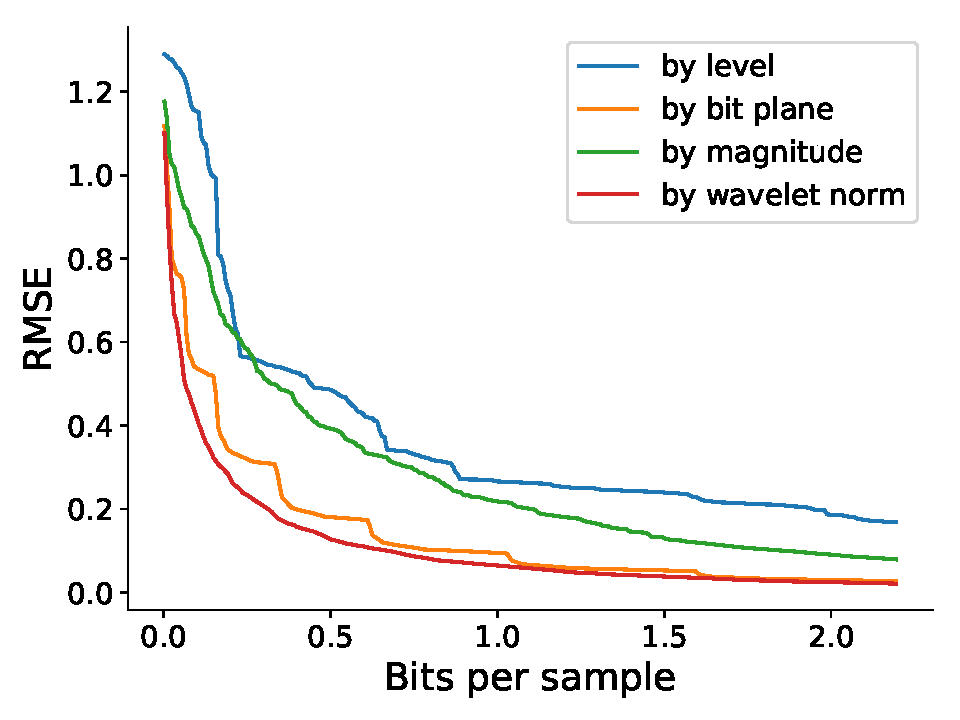
\includegraphics[width=0.48\linewidth]{img/motivation/motivation-psnr-turbulence.pdf}}
	\subcaptionbox{Plasma}
 	{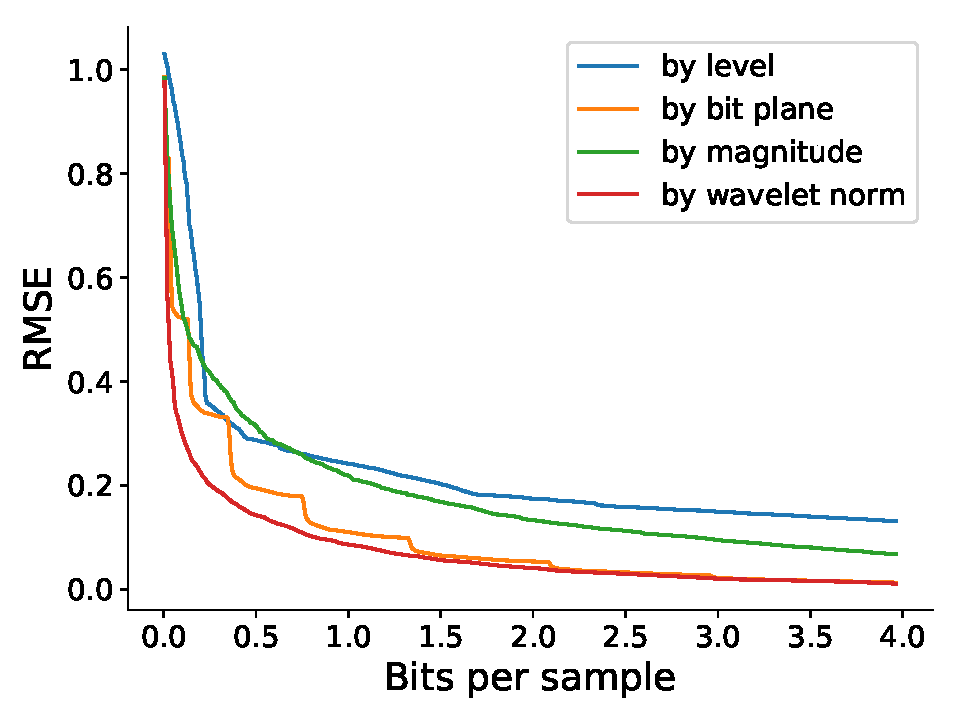
\includegraphics[width=0.48\linewidth]{img/motivation/motivation-psnr-plasma.pdf}}
	\subcaptionbox{Velocity-z}
 	{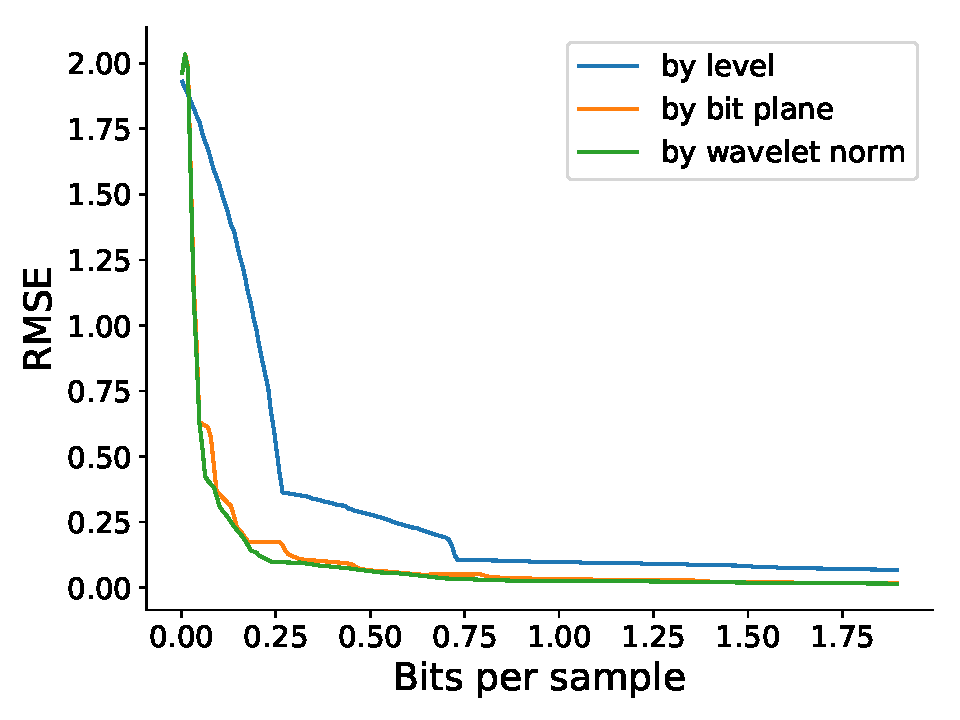
\includegraphics[width=0.48\linewidth]{img/motivation/motivation-psnr-velocityz.pdf}}
 	\caption{Root-mean-square error of reconstructed functions using the three data-agnostic streams
 	defined in Section \ref{sec:motivation}. Lower is better. The streams are truncated to highlight
 	the differences, without omitting important information. \emph{by wavelet norm} performs best,
 	followed closely by \emph{by bit plane}.}
 	\label{fig:motivation-rmse}
\end{figure}

\begin{figure}[h]
  \centering
	\subcaptionbox{Boiler}
  {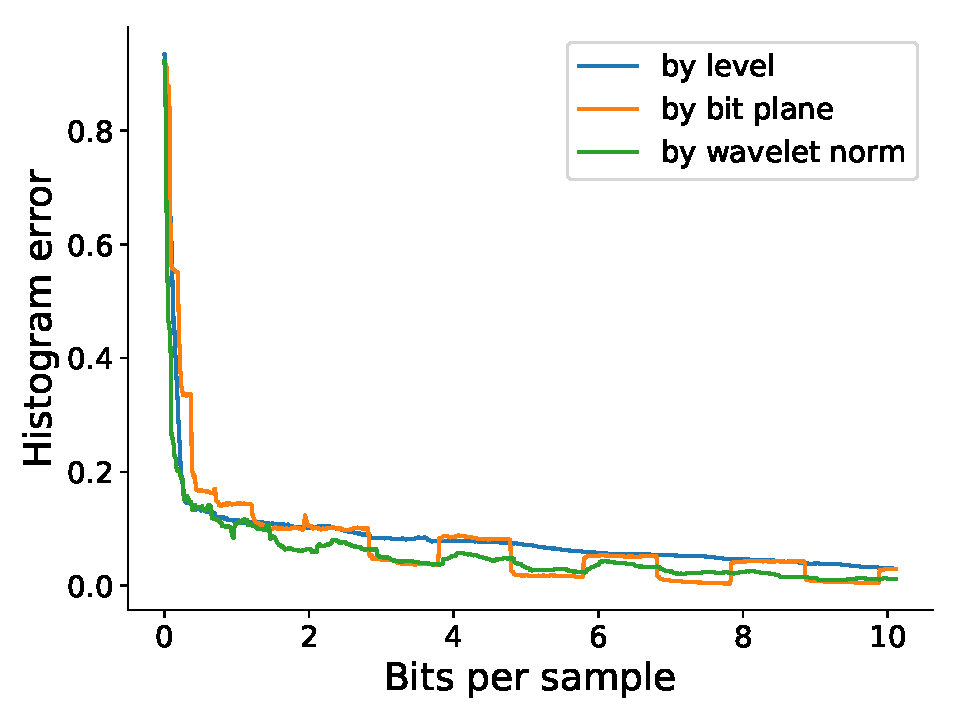
\includegraphics[width=0.48\linewidth]{img/motivation/motivation-histogram-boiler.pdf}}
	\subcaptionbox{Diffusivity}
 	{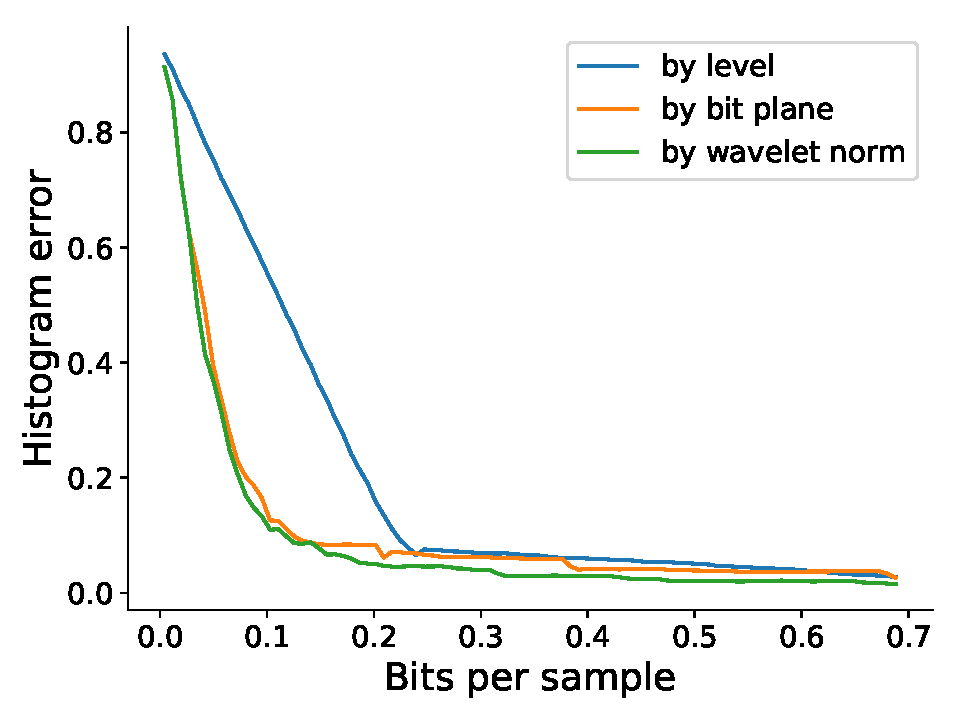
\includegraphics[width=0.48\linewidth]{img/motivation/motivation-histogram-diffusivity.pdf}}
	\subcaptionbox{Euler}
 	{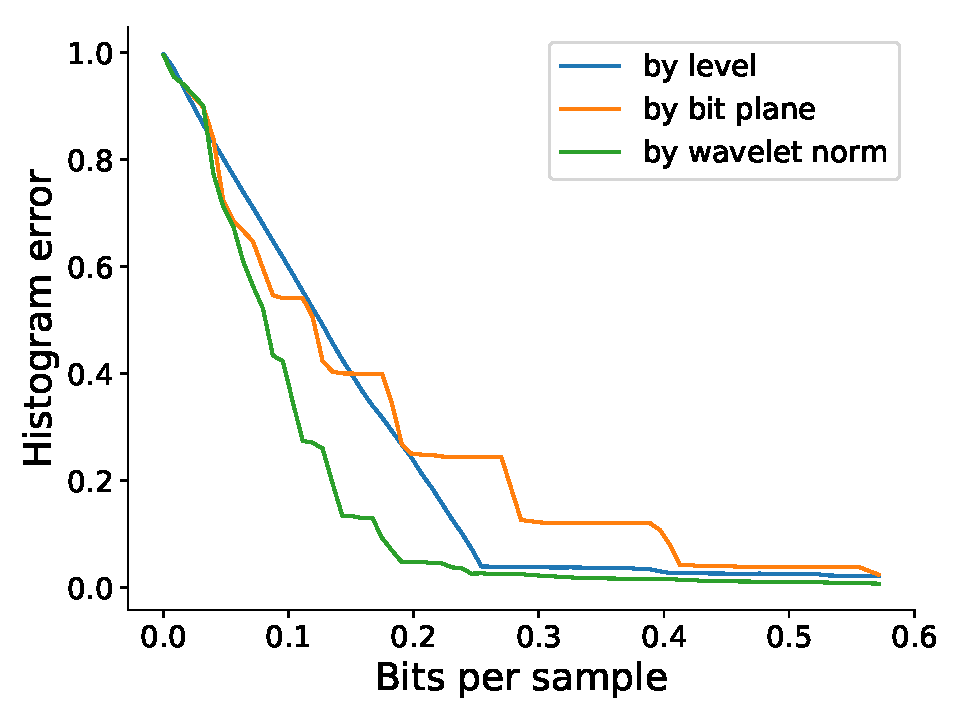
\includegraphics[width=0.48\linewidth]{img/motivation/motivation-histogram-euler.pdf}}
	\subcaptionbox{Turbulence}
 	{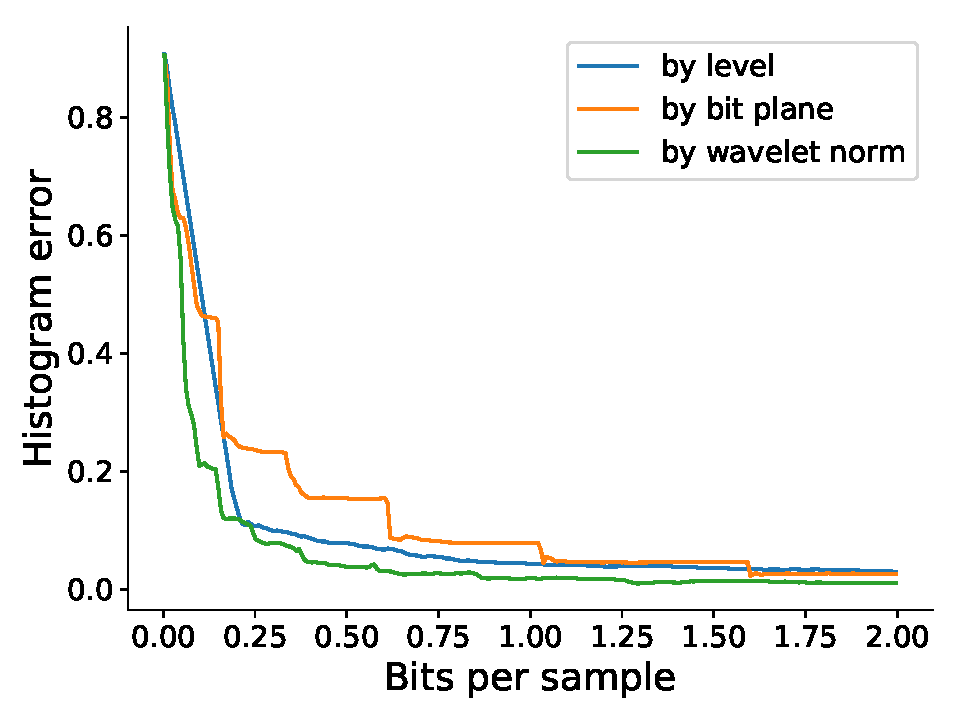
\includegraphics[width=0.48\linewidth]{img/motivation/motivation-histogram-turbulence.pdf}}
	\subcaptionbox{Plasma}
 	{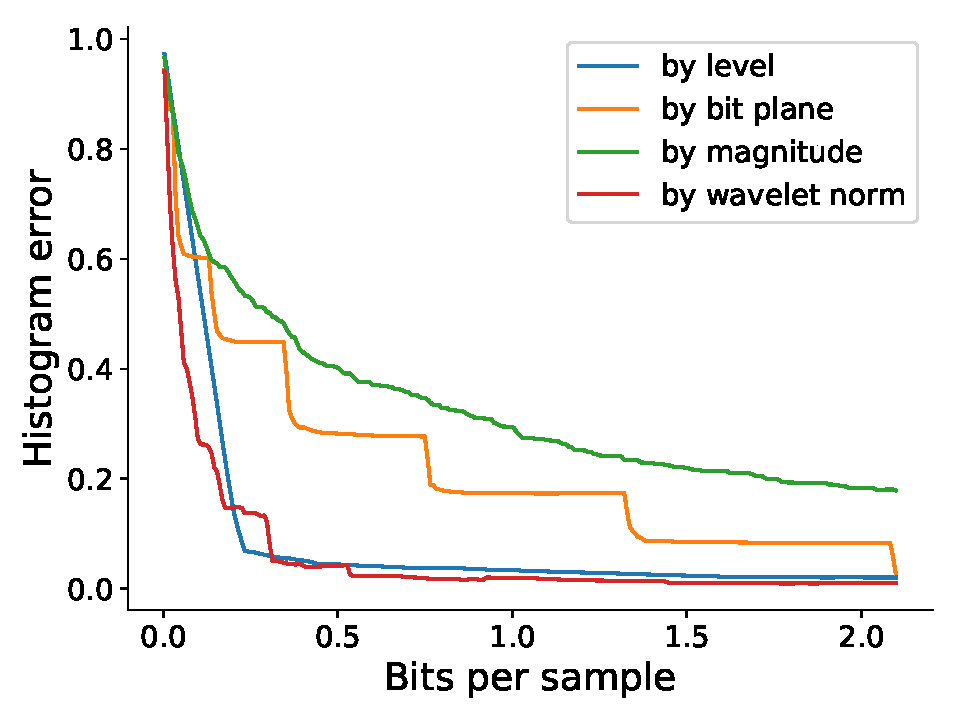
\includegraphics[width=0.48\linewidth]{img/motivation/motivation-histogram-plasma.pdf}}
	\subcaptionbox{Velocity-z}
 	{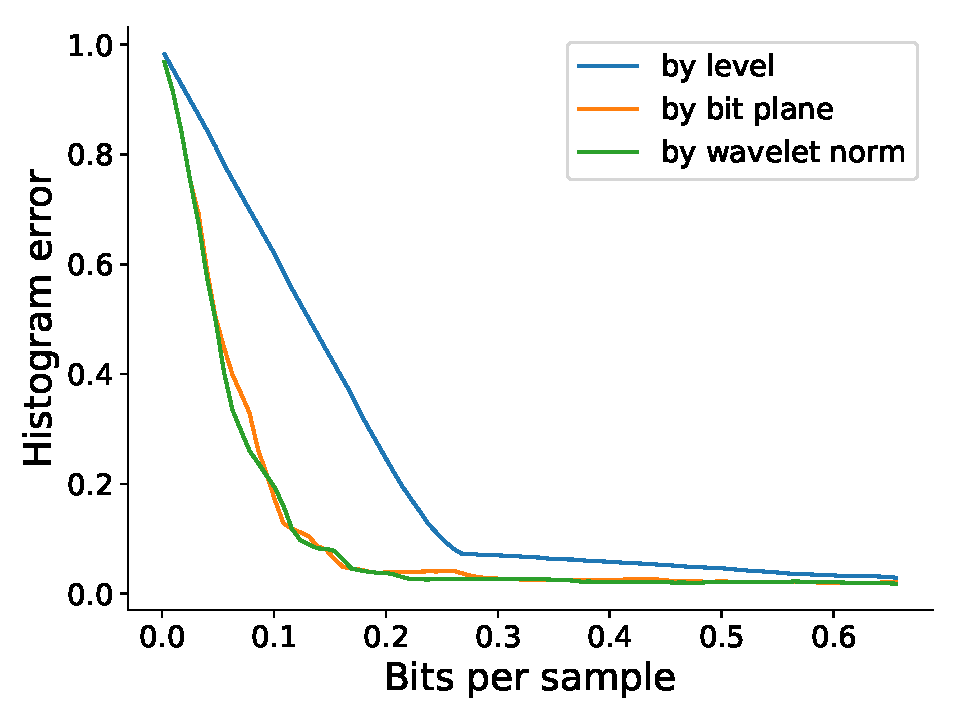
\includegraphics[width=0.48\linewidth]{img/motivation/motivation-histogram-velocityz.pdf}}
 	\caption{Histogram error of reconstructed functions using the three data-agnostic streams defined
 	in Section \ref{sec:motivation}. Lower is better. Each histogram comprises of 256 bins. The
 	streams are truncated to highlight the differences, without omitting important information.
 	\emph{by wavelet norm} performs best.}
 	\label{fig:motivation-histogram}
\end{figure}

\begin{figure}[h]
  \centering
	\subcaptionbox{Boiler, isovalue = $0.07$}
  {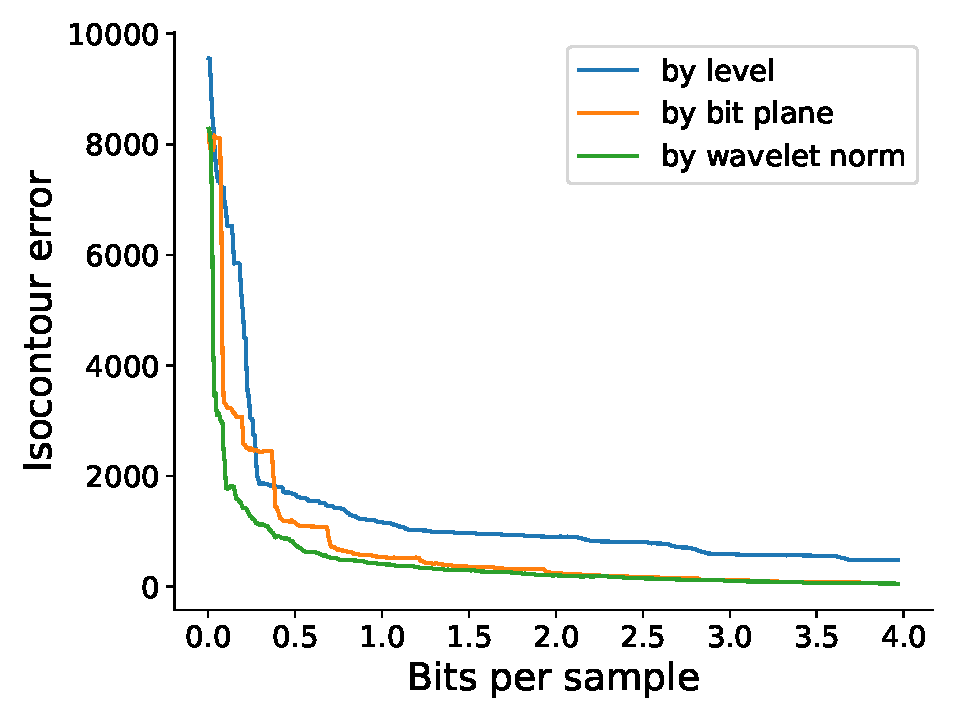
\includegraphics[width=0.48\linewidth]{img/motivation/motivation-isocontour-boiler.pdf}}
	\subcaptionbox{Diffusivity, isovalue = $0.04315$}
 	{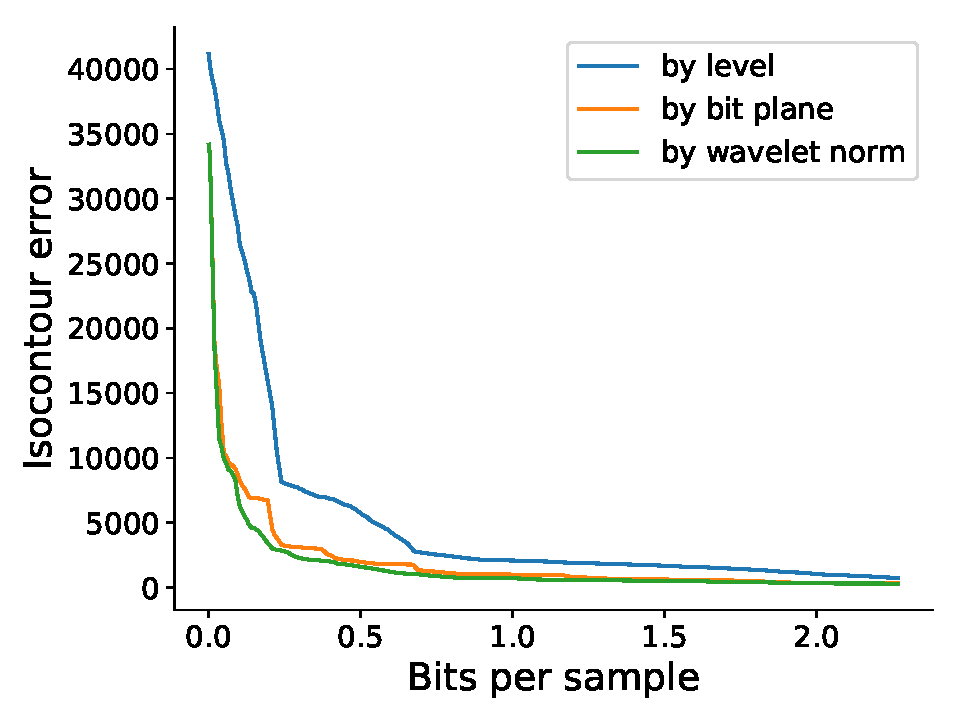
\includegraphics[width=0.48\linewidth]{img/motivation/motivation-isocontour-diffusivity.pdf}}
	\subcaptionbox{Euler, isovalue = $3$}
 	{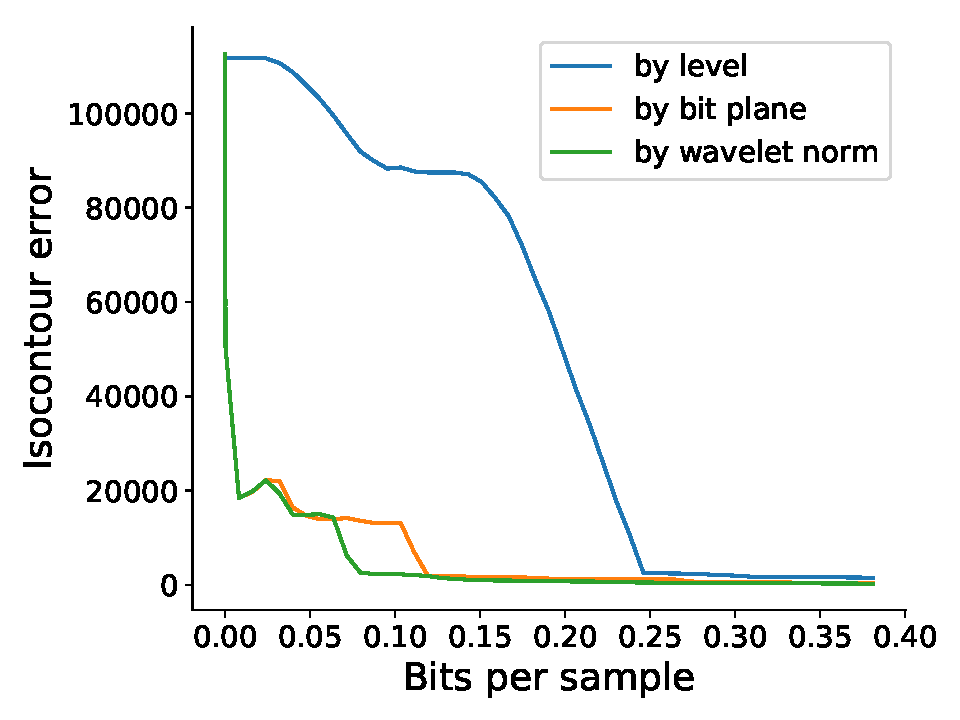
\includegraphics[width=0.48\linewidth]{img/motivation/motivation-isocontour-euler.pdf}}
	\subcaptionbox{Turbulence, isovalue = $2$}
 	{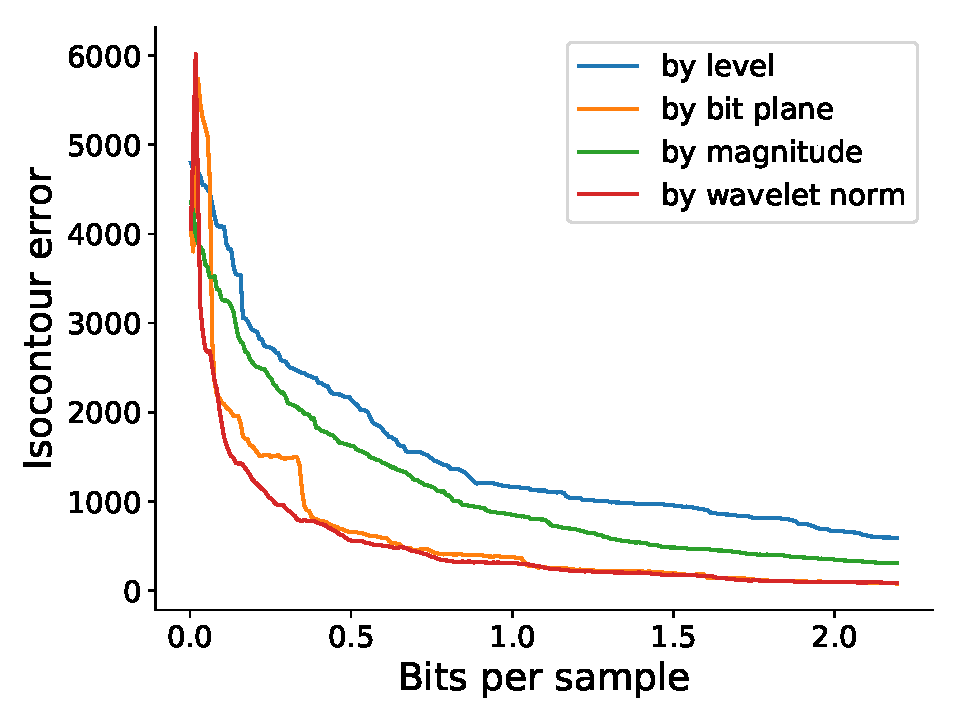
\includegraphics[width=0.48\linewidth]{img/motivation/motivation-isocontour-turbulence.pdf}}
	\subcaptionbox{Plasma, isovalue = $2$}
 	{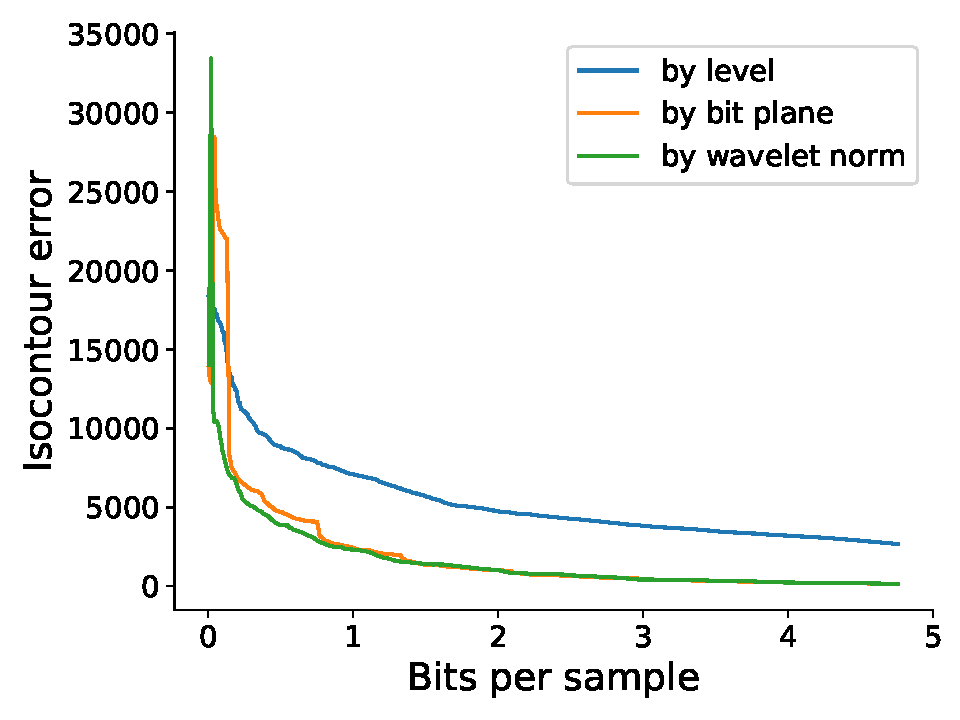
\includegraphics[width=0.48\linewidth]{img/motivation/motivation-isocontour-plasma.pdf}}
	\subcaptionbox{Velocity-z, isovalue = $-2$}
 	{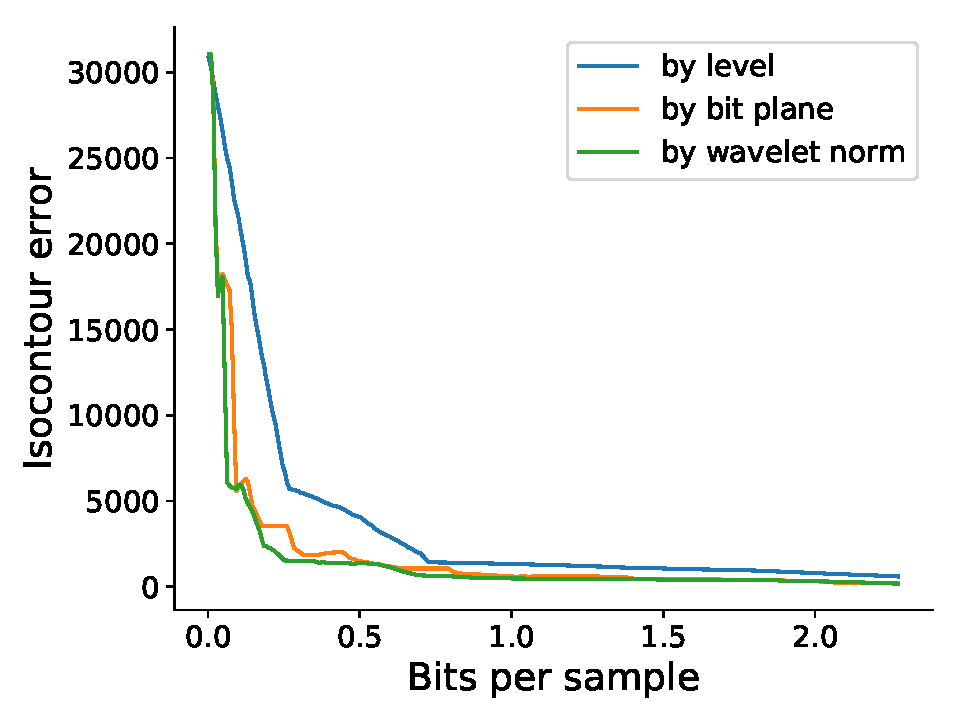
\includegraphics[width=0.48\linewidth]{img/motivation/motivation-isocontour-velocityz.pdf}}
 	\caption{Isocontour error of reconstructed functions using the three data-agnostic streams defined
 	in Section \ref{sec:motivation}. Lower is better. The streams are truncated to highlight the
 	differences, without omitting important information. \emph{by wavelet norm} performs best.}
 	\label{fig:motivation-isocontour}
\end{figure}

We see that, for all metrics, the \emph{by wavelet norm} stream consistently performs the
best. The \emph{by bit plane} works almost as well as \emph{by wavelet norm} for RMS error and
isocontour error, but not for histogram error. The \emph{by level} stream works poorly in almost all cases.
These results show that it is often suboptimal to stream or reduce data exclusively in either
resolution or precision. Combining these two dimensions of data reduction can lead to significant
quality improvement at the same bit rate, especially when quantities of interest other than simply
the function itself are considered. The reason is that \emph{by wavelet norm} can take advantage of
the fact that a higher-ordered bit from a fine-scale coefficient could contribute more than a
lower-ordered bit from a coarse-scale coefficient (which \emph{by level} ignores), and vice-versa
(which \emph{by bit plane} ignores). It is unclear, however, whether \emph{by wavelet norm} is the
best stream to use in all cases. To answer this question, we will expand our study from
data-agnostic to data-dependent streams that are optimized for each of these quantities of interest.
While data-dependent streams are likely unrealizable in practice due to the fact that the
`'receiver'' of data does not have access to the data beforehand, we hope they provide insights for
designing streams that improve on the generic \emph{by wavelet norm}, by being tailored to each
error metric.

\subsection{Data-dependent, quantity-optimized streams}
\label{sec:data_dep_streams}

This section aims to solve the problem of finding the most optimal (and data-dependent) stream
possible, given a data set and an error metric. An error metric is a function $E(Q(f'),Q(f))$, where
$f$ is the original data field and $f'$ is a reconstructed version of $f$ using a subset of the
bits. $Q$ is an operation that trasnforms a raw data fields (e.g., $f$ and $f'$) to some quantity of
interest (e.g., derivatives, histograms, isocontours, etc). There can be multiple error functions
$E$ that makes sense for the same quantity $Q$. In this paper, we choose to use only one error
metric with each quantity, one which we believe is either common, or intuitive and simple without
sacrificing generalizability. The list of quantity-optimized streams studied in this paper includes
\emph{rmse-optimized} (Section [REF]), \emph{gradient-optimized} (Section [REF]),
\emph{laplacian-optimized} (Section [REF]), \emph{histogram-optimized} (Section [REF]), and
\emph{isocontour-optimized} (Section [REF]).

Studying a (data-dependent) quantity-optimized stream is important because such a stream serves both
as a benchmark, and a source of insights for other, more practical streams for the same quantity.
One way to define the ``optimal'' stream for a quantity $G$ could be the stream that incurs the
minimum error $E$ at every point. However, in trying to realize it, our experience has been that
such a stream does not exist. Assume otherwise that the optimal stream exists, then by its
definition, it must be possible to construct it using the following greedy algorithm: start with a
pool of all the chunks (and correspondingly an all-zero $f'$ and a presumably very high $E$), pick
the chunk that when enabled, would minimize $E$, remove it from the pool. Repeatedly pick the next
chunk that minimizes $E$, until the pool is empty. Running this algorithm, we have noticed that
there can be a situation in which the next chunk that minimizes the error is on a low-order bit
plane of a very fine-scale coefficient, which contributes little to the reconstructed function. The
error is minimized because it is kept approximately constant. In this case it is actually better to
pick a chunk that increases the error, but otherwise contributes a lot more to the reconstructed
function. In optimization terms, it is necessary to move in a direction that increases the error to
avoid getting stuck in a local minima.

The optimal stream for an error metric can also be defined as the stream such that the area bounded
by its plotted error curve and the horizontal axis is smallest. However, the usefulness of such a
definition is limited in practice, because a stream should be able to be terminated at any point and
still be expected to produce as small of an error as possible. Instead, we observe that the greedy
algorithm stated in the paragraph above can be slightly modified to avoid the problem of being stuck
in local minima. We start with a pool consisting of all the chunks and an empty stream, and build
the stream back to front. In each step, the chunk whose removal from the pool has the least impact
on the error $E$ is removed and inserted to the beginning of the current stream. This algorithm
solves the problem of unimportant chunks being picked too early in the original algorithm, because
here, being picked early means they would be at the end of the stream, instead of the beginning.

In our experience, however, the back-to-front greedy algorithm is too costly in practice. Ignoring
all the steps done in each iteration, this algorithm amounts to an $n^2$-iteration, 2-level nested
loop, where $n$ is the number of chunks. In 2D, with a $256^2$ data set, a chunk size that spans
$16$ coefficients, and $16$ bits of quantization, the total number of chunks would be $n=65536$, and
$n^2$ would be in the billions, which we have found to be prohibitively large. We have therefore
adopted a simplified version of this algorithm, where only one pass through the chunks are needed.
Our modified algorithm disables (sets to zero) a new chunk $c_i$ in each iteration, computes and
records the error $E_i$ due to chunk $c_i$ missing, and enables again the chunk at the end of the
iteration. After $n$ iterations, each chunk has an associated weight, $E_i$. The optimal stream,
then, is simply a sorted list of chunks, in decreasing order of the weights. In our experience, this
simplified algorithm brings the running time down from days to minutes, while retaining the same
performance.
\section{Data dependent task-optimized streams}
\label{sec:data_dep_streams}

The previous section used fixed ordered streams, either by bit plane, level, or wavelet norm. We
will show that these streams are suboptimal, and will describe a greedy heuristic to obtain better stream
tailored to a task. 

\subsection{Motivation}
To test whether a stream that is suited to a certain task (function reconstruction, using PSNR as
the metric) also performs well in another (histogram computation), we compare the streams introduced
in the previous section using a histogram error metric that is the Earth Mover Distance (EMD)~\cite{emd1998}.
The EMD measures how far the histogram of the reconstructed data is from the histogram of
the original data. We use 256 histogram bins in all experiments. The results are shown in Figure
\ref{fig:histogram-motivation}. Compared to Figure \ref{fig:motivation}, the \emph{by level} stream
is removed and two other streams are added: \emph{resolution-adaptive, EMD-optimized} and
\emph{fully adaptive, EMD-optimized}. The two new streams are analogous to their RMSE counterparts
(i.e., the two data-dependent streams in Figure \ref{fig:motivation}, now renamed to
\emph{resolution-adaptive, RMSE-optimized} and \emph{fully adaptive, RMSE-optimized}), but are
computed by greedily minimizing EMD instead of RMSE with regards to the ground truth.

\begin{figure}
	\centering
	\subcaptionbox{Magnetic}
	{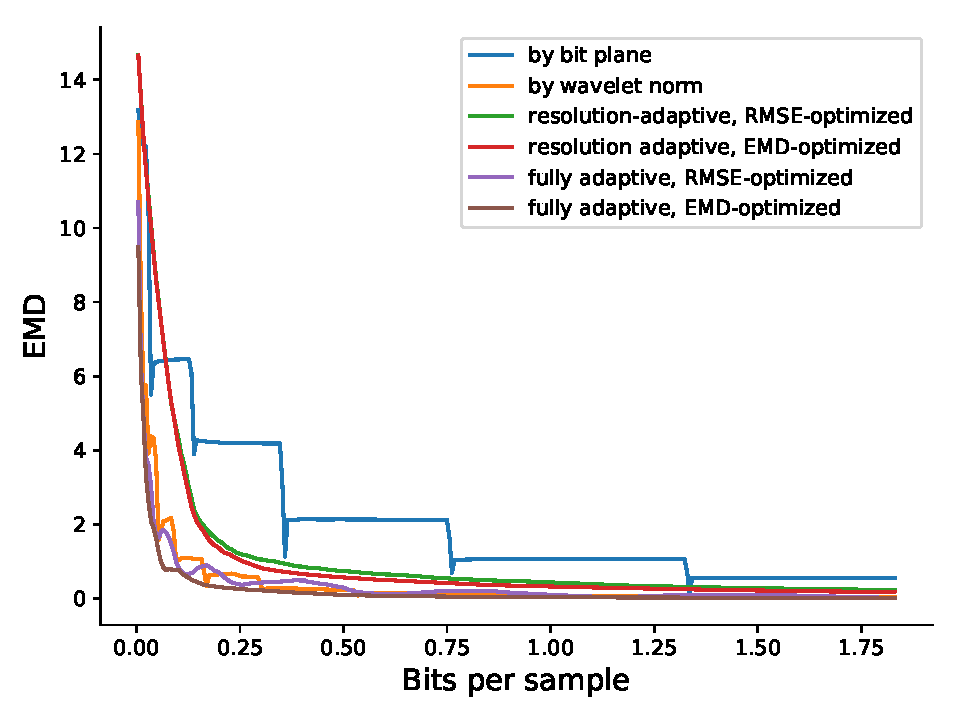
\includegraphics[width=0.44\linewidth]{img/motivation/magnetic-histogram-motivation.pdf}}
	\subcaptionbox{Boiler-O2}
	{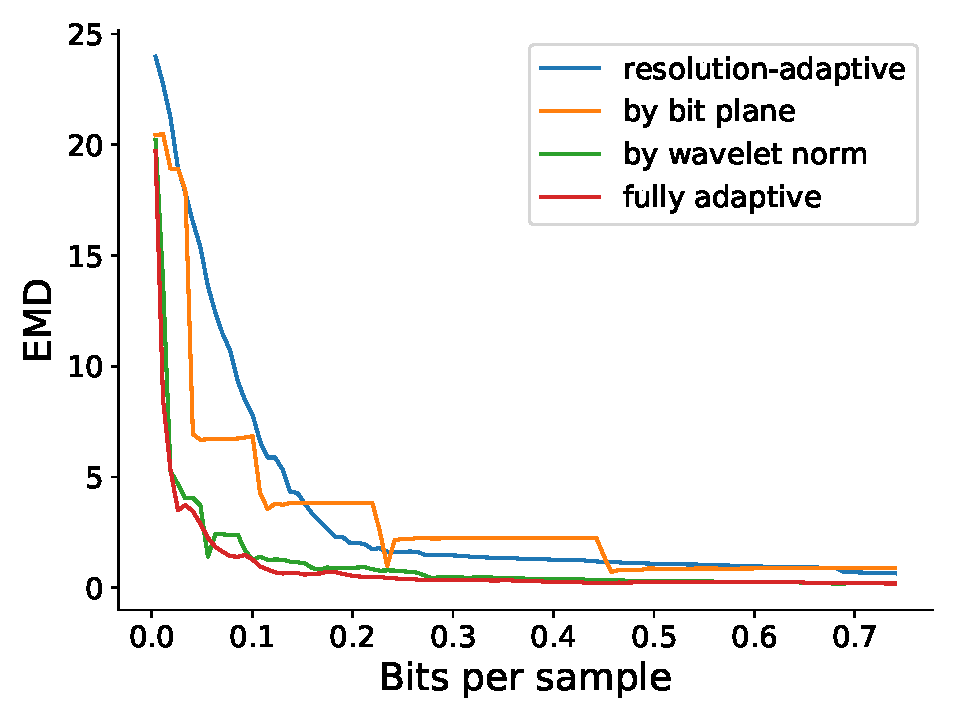
\includegraphics[width=0.44\linewidth]{img/motivation/boiler-histogram-motivation.pdf}}
	\subcaptionbox{Flame-OH}
	{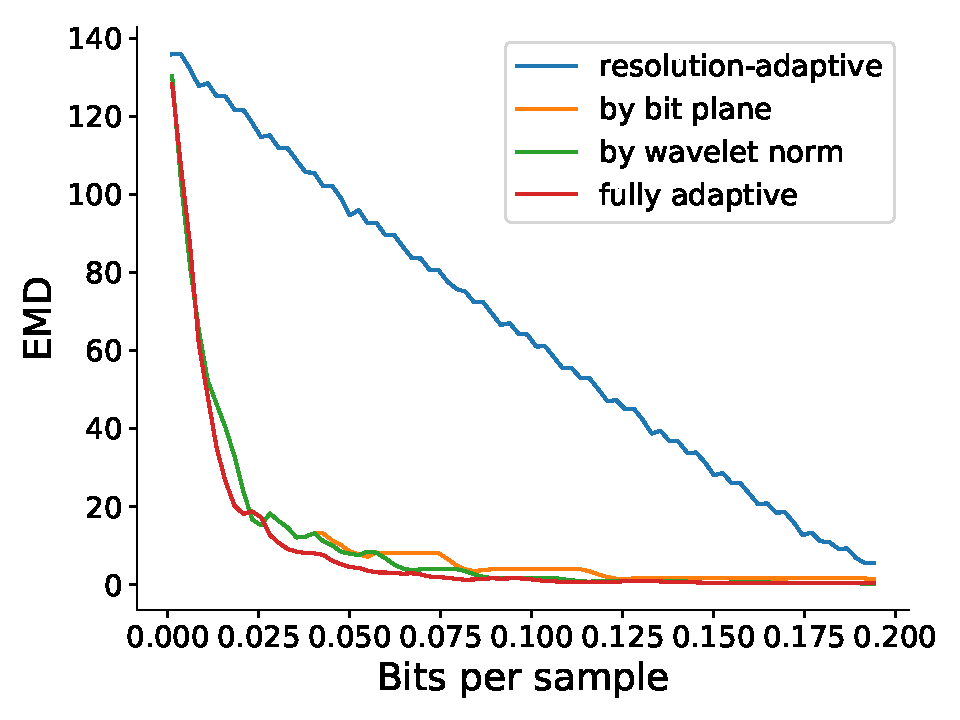
\includegraphics[width=0.44\linewidth]{img/motivation/kflame-oh-histogram-motivation.pdf}}
	\subcaptionbox{Miranda-diffusivity}
	{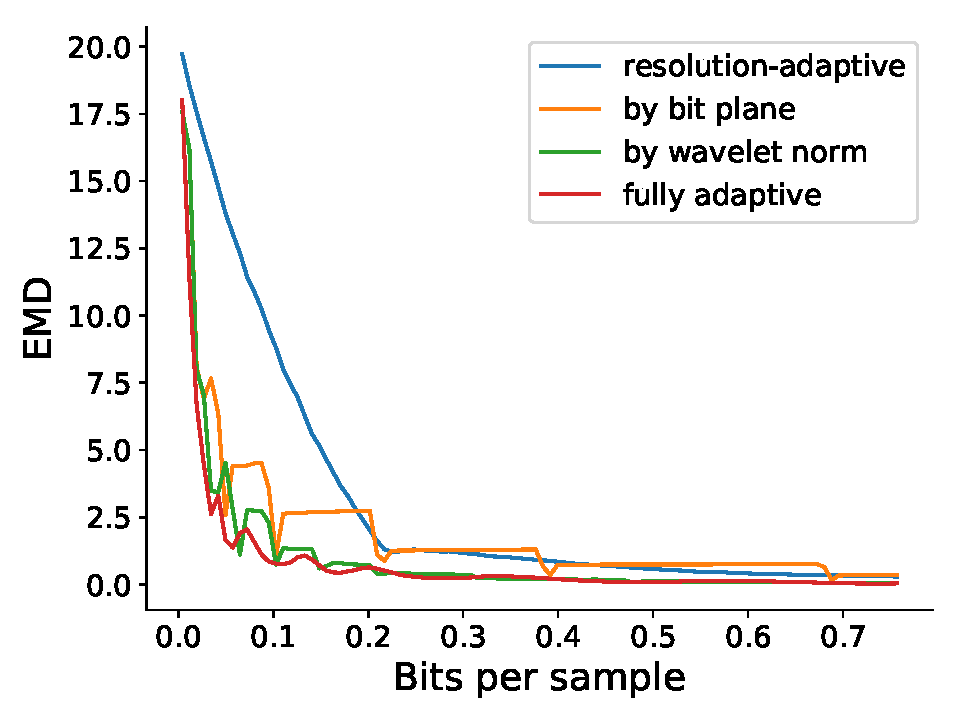
\includegraphics[width=0.44\linewidth]{img/motivation/diffusivity-histogram-motivation.pdf}}
	\caption{Histogram error comparison. Lower EMD is better. The streams are truncated	towards the
	end where the errors become negligibly small.}
	\label{fig:histogram-motivation}
\end{figure}

The \emph{by bit plane} and \emph{by wavelet norm} streams match one another closely in terms of
PSNR, but differ significantly in EMD. Furthermore, the \emph{fully adaptive, RMSE-optimized} stream
underperforms  \emph{fully adaptive, EMD-optimized}, indicating that recontructing an accurate
function and reconstructing an accurate histogram require two very different orderings of bits.
Figure \ref{fig:histogram-comparison} illustrates how a quantitative difference in EMD translates to
a visual difference in histogram.

\begin{figure}
	\centering
	\subcaptionbox{\emph{by bit plane}}
	{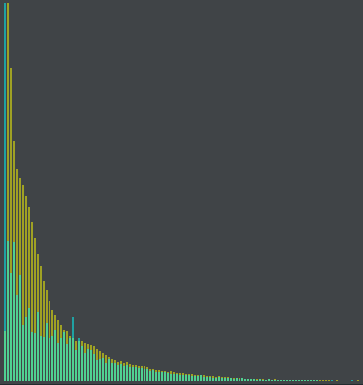
\includegraphics[width=0.24\linewidth]{img/motivation/histogram-by-bit-plane.png}}
	\subcaptionbox{\emph{by wavelet norm}}
	{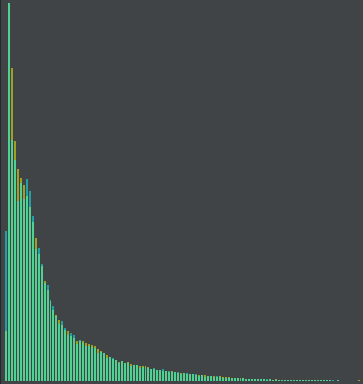
\includegraphics[width=0.24\linewidth]{img/motivation/histogram-by-wavelet-norm.png}}
	\subcaptionbox{\emph{fully adaptive, RMSE-optimized}}
	{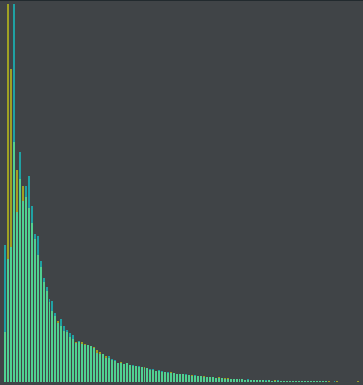
\includegraphics[width=0.24\linewidth]{img/motivation/histogram-rmse-optimized.png}}
	\subcaptionbox{\emph{fully adaptive, EMD-optimized}}
	{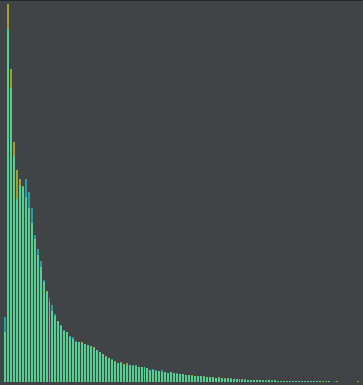
\includegraphics[width=0.24\linewidth]{img/motivation/histogram-emd-optimized.png}}
	\caption{Histogram comparison for the Magnetic data set at 0.16 bits per sample. The reconstructed
	histogram (blue) is blended with the ground truth histogram (yellow), so green is where the two
	overlap. Larger overlap (more green, less blue and yellow) is better.}
	\label{fig:histogram-comparison}
\end{figure}



\subsection{Computation}
In~\Cref{sec:combining} we demonstrated that different tasks may need different streams. For example,
PSNR stream significantly underperforms the histogram stream when applied to the histogram
query~(\Cref{fig:histogram-comparison}).
Unfortunately, there is no single definition of best stream is for a given query. It could be a stream that
exhibit small changes in the data or stream that reaches the smallest error fastest.
Moreover, it is common to stop the streaming in case the quantity of interest is good enough or the data size
reached the limit of the machine.

We define the best stream as
a sequence of refinements that reach the minimum error at given stopping bit budget. Alas, in interactive application
we can only make assumptions what will be the number of bits streamed before user decides to stop the streaming. For
example, if a user drasticly changes viewpoint in a volume rendering application, the stream starts almost from scratch.
Taking the lack of control over the stopping budget to the extreme, the best stream becomes the one which minimizes
the error at all bit budgets. However, as in any optimization problem we may reach local minimum, as
chunks that improve the error but have impact on later refinement will have lower priority. The existence of local
minima prevents this progressive stream to be globally optimal.
We can compute the optimal stream by searching the ordering space for one that is optimal for the largest number
of bit budgets. Unfortunately, finding such ordering is exponential in number of chunks. Therefore, we focus on
finding a greedy scheme that could be good representative for the optimal stream. There are two primary directions
along which we can greedily search for sream: fine-to-coarse or coarse-to-fine.

\paragraph*{Fine-to-coarse greedy algorithm} utilizes full dataset to construct the stream.
Moreover,
if we wanted to precompute stream order which could be utilized during query, we would have access to whole
data set and could compute this stream. The algorithm is in principle a reverse of the previous approach, the
stream is constructed by starting with full data set and one by one disabling the chunks. At each step, a chunk
with smallest errorr impact is disabled (TODO: more detail). This algorithm is still of greedy nature as it
makes only locally optimal choice.
The running time of this algorithm is $O(n^3)$ as we start with $n$ chunks
and at each streaming step decrease the chunk count by one. The cube factor comes from the need to perform inverse
wavelet transform and compute the error for each chunk.

\begin{algorithm}
  \KwData{slice, unordered list of chunks}
  \KwResult{ordered list of chunks with decreasing error}
  orderedChunks = $\emptyset$\;

  \While{$|$chunks$| \ne 0$}{
   smallestChunk = front(chunks)\;
   \For{chunk $\in$ chunks}{
     sliceCopy = slice\;
     disableChunk(sliceCopy, chunk)\;
     error = computeError(sliceCopy, slice)\;
     \If{error $<$ error(smallestChunk)}{
       smallestChunk = chunk\;
     }
   }

   disableChunk(slice, smallestChunk)\;
   chunks = chunks $\setminus$ smallestChunk\;
   orderedChunks = orderedChunks $\cup \{$smallestChunk$\}$\;
  }
  \caption{Fine-to-coarse stream optimization algorithms}
\end{algorithm}

\begin{figure}
        \centering
        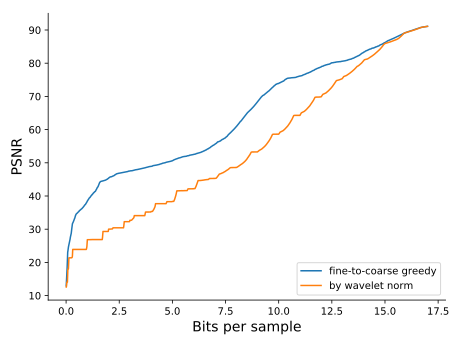
\includegraphics[width=0.48\linewidth]{img/figure4_new/rmse-miranda-viscosity}
        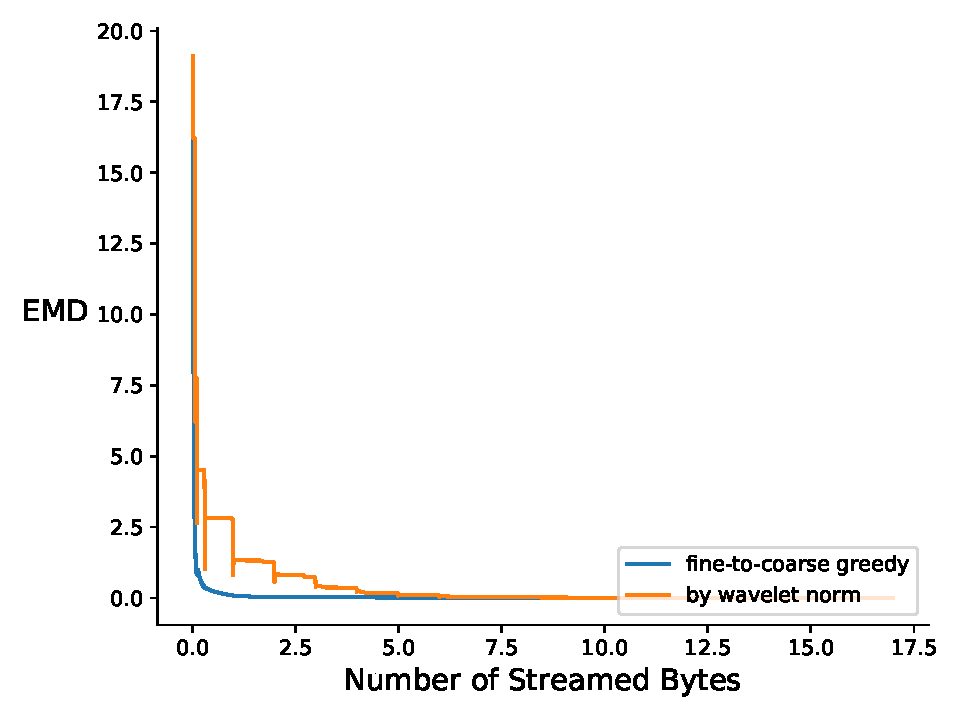
\includegraphics[width=0.48\linewidth]{img/figure4_new/histogram-miranda-viscosity}
        \caption{Comparison of fine-to-coarse and by wavelet norm streams on Miranda viscosity data set.
                 On the left is stream optimized for PSNR (higher is better) and on the right for histogram (lower is better).
                 Despite using larger block size for the greedy stream ($16 \times 16$) due to performance reasons, it still
                 significantly outperforms the by wavelet norm stream for both quantities.}
\end{figure}


\paragraph*{Coarse-to-fine greedy algorithm} starts with no data and
the initial error is computed with respect to the full data set. Then
it takes a list of all chunks in the dataset, computes the error as if
the chunk was enabled, and picks the chunk with the highest absolute
difference in the error with respect to the current error.  We use
absolute difference to avoid the case where the error difference is
zero or negative, which would result in a long stream of chunk that do
not decrease the error significantly. \ptb{I am not sure in understand
  the previous sentence} This assumption reflects the expectation of
more data meaning better result. Similarly to the coarse-to-fine
algorithm, the running time is still $O(n^3)$.


Since the fine-to-coarse greedy stream outperforms the coarse-to-fine stream we further investigate possible
runtime optimizations. Surprisingly, performing only the first round of chunk error calculation and then sorting
those chunks by the error closely matches the full greedy algorithm. This simple optimization reduces the time
complexity to $O(n^2)$ and thus makes it more practical. We use this greedy scheme throught our evaluation named
\emph{fully adpative} stream.

\begin{figure}
        \centering
        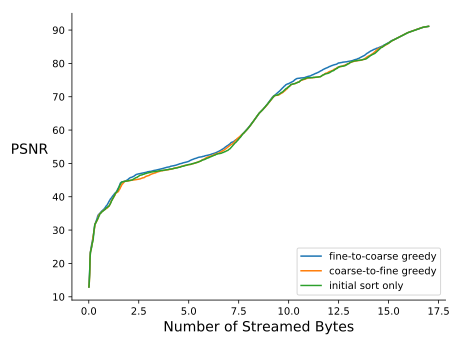
\includegraphics[width=0.48\linewidth]{img/figure6/rmse-miranda-viscosity}
        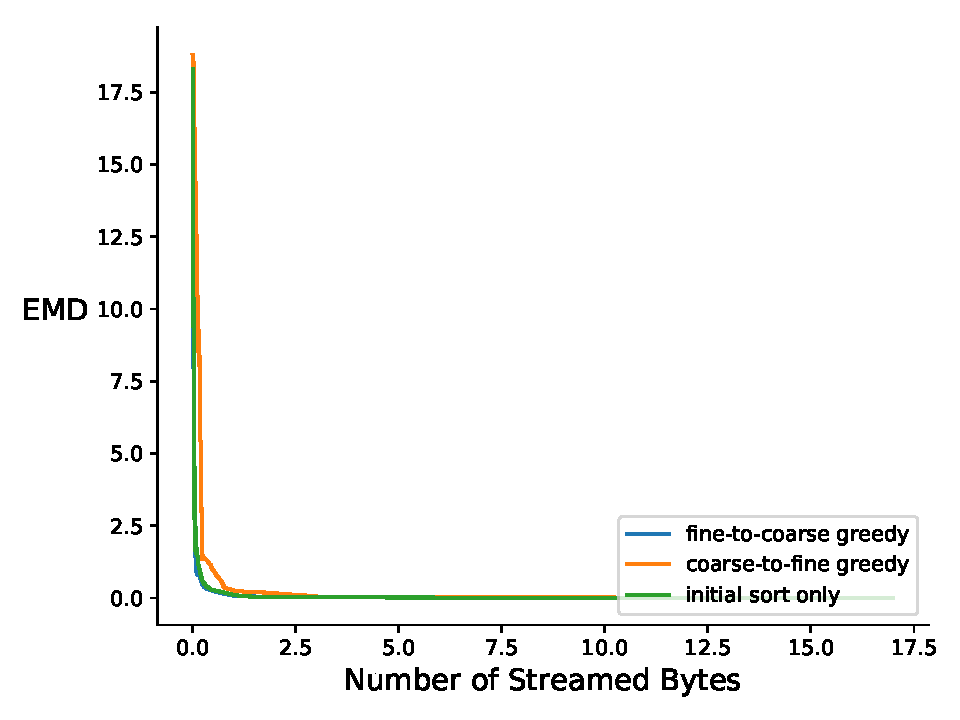
\includegraphics[width=0.48\linewidth]{img/figure6/histogram-miranda-viscosity}
        \caption{The fully adaptive stream (fine-to-coarse with only initial sorting) closely follows the coarse-to-fine and
                 fine-to-coarse streams both for PSNR and histogram.}
\end{figure}

%%% Local Variables:
%%% mode: latex
%%% TeX-master: "template"
%%% End:

\subsection{Derivative Computation} \label{sec:derivatives}

Computation of derivative-based quantities is important in data analysis. In this paper, derivatives
are always computed using finite differences, which is common in practice. We use 32 bits for
quantization in this section to ensure enough precision for finite differences, as compared to 16
bits for other experiments. We always compute finite differences on the finest resolution grid to
avoid computing distances between quantities defined on grids of different resolutions.

\subsubsection{Gradient Computation} \label{sec:gradient}

\begin{figure*}[t]
\centering
\subcaptionbox{\emph{boiler}}{%
{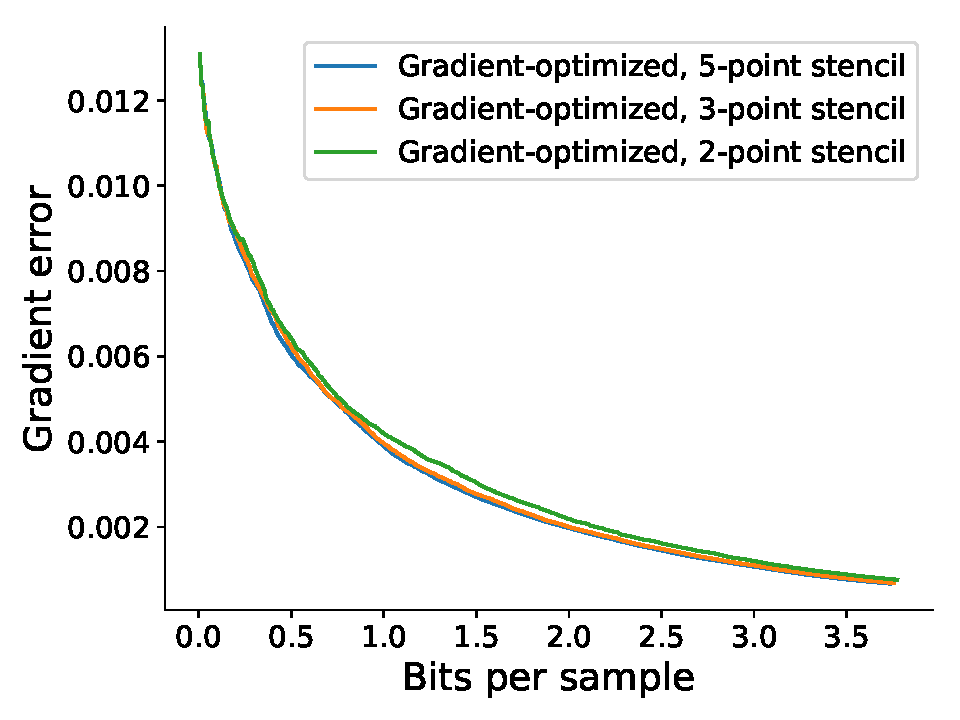
\includegraphics[width=0.24\linewidth]{gradient/gradient-optimized-boiler}}}
\subcaptionbox{\emph{diffusivity}}{%
{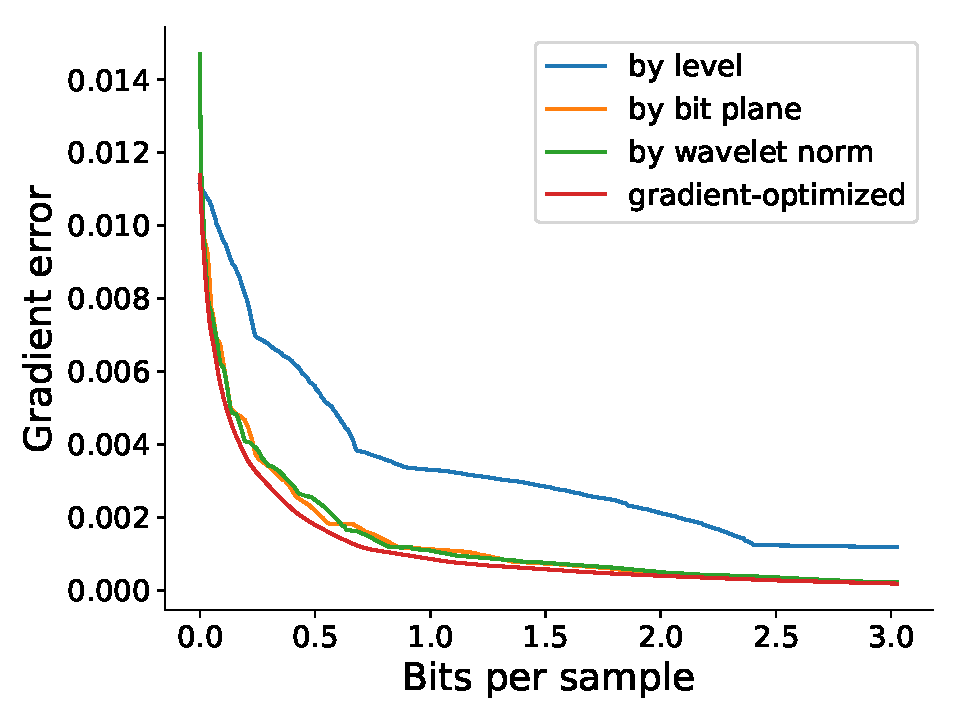
\includegraphics[width=0.24\linewidth]{gradient/gradient-optimized-diffusivity}}}
\subcaptionbox{\emph{turbulence}}{%
{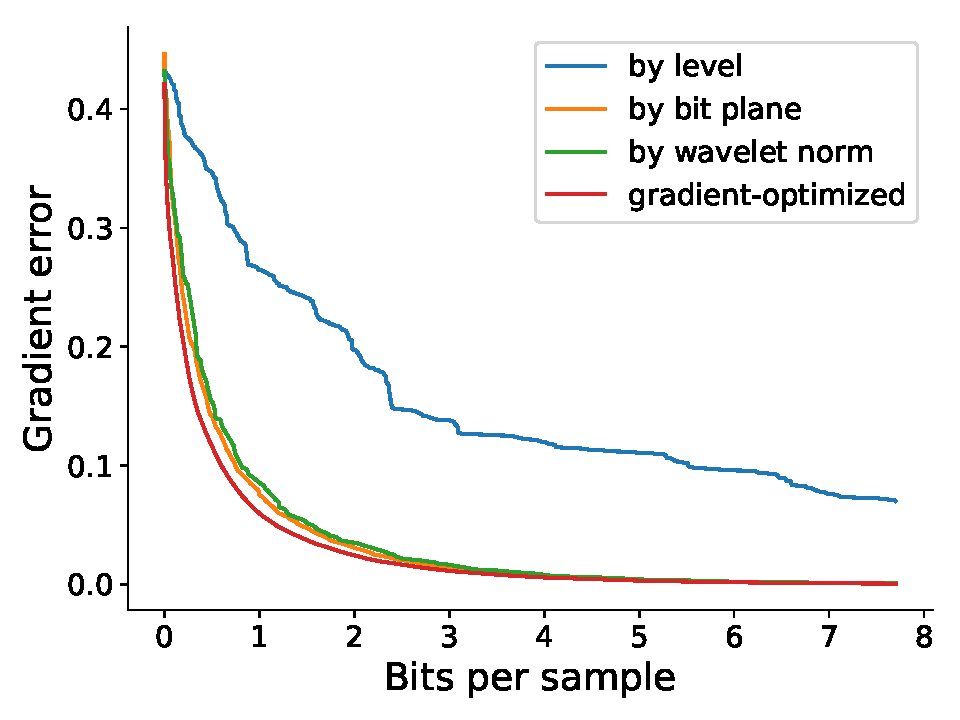
\includegraphics[width=0.24\linewidth]{gradient/gradient-optimized-turbulence}}}
\subcaptionbox{\emph{pressure}}{%
{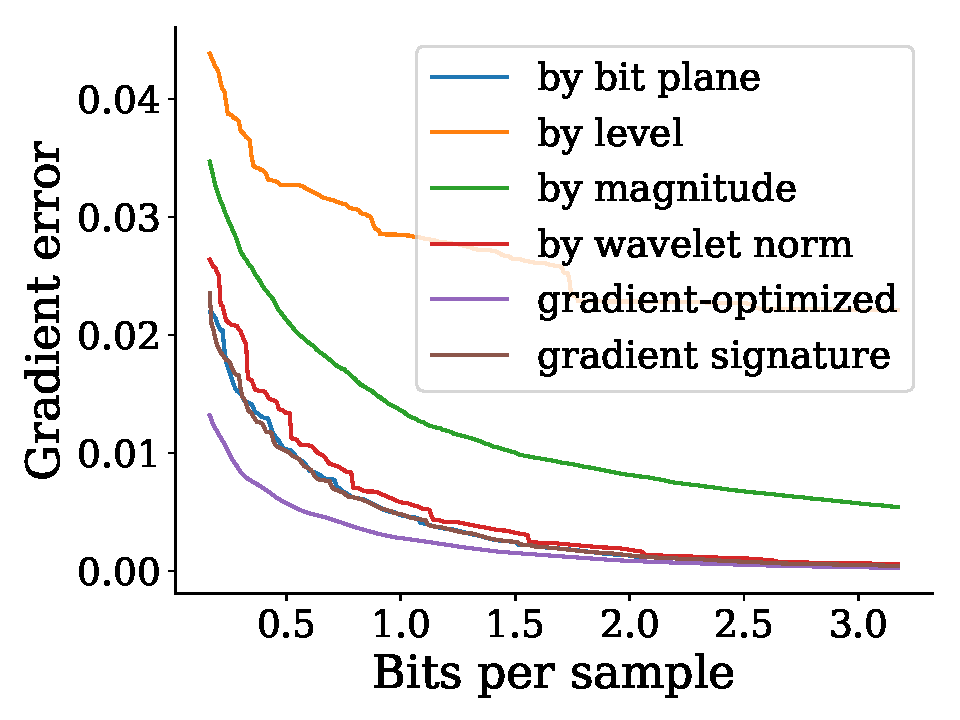
\includegraphics[width=0.24\linewidth]{gradient/gradient-optimized-pressure}}} 
\caption{Gradient error of reconstructed functions. Lower gradient error is better. Leading zero
packets are removed, and the plots are truncated in the same way as in~\Cref{fig:rmse-optimized}.
The trend in error, in all cases, is $\sgop < \sgsg \approx \sbit < \swav < \smag < \slvl$.}
\label{fig:gradient-error-comparison}
\vspace{1em}

\centering
\subcaptionbox{\emph{by level} (\slvl)}{%
{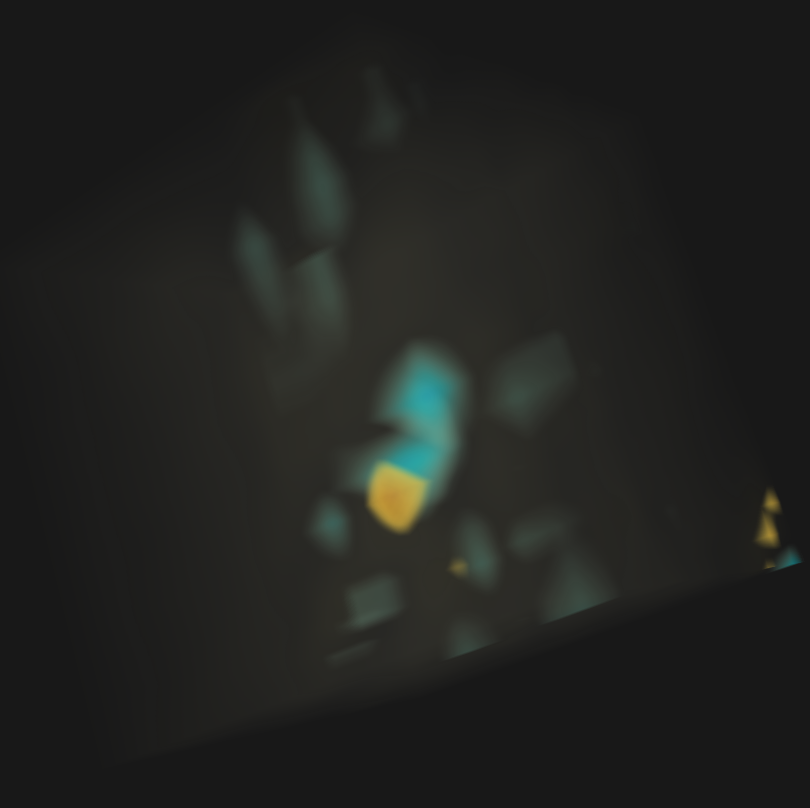
\includegraphics[width=0.16\linewidth]{gradient/gradient-turbulence-level}}}
\subcaptionbox{\emph{by bit plane} (\sbit)}{%
{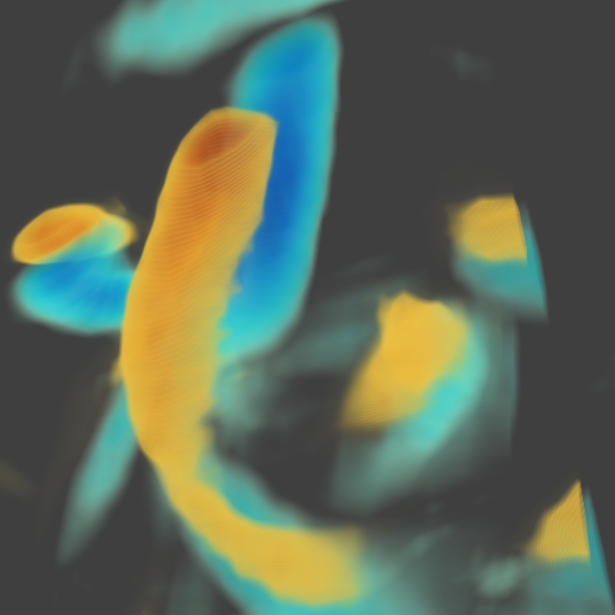
\includegraphics[width=0.16\linewidth]{gradient/gradient-turbulence-bit-plane}}}
\subcaptionbox{\emph{by wavelet norm} (\swav)}{%
{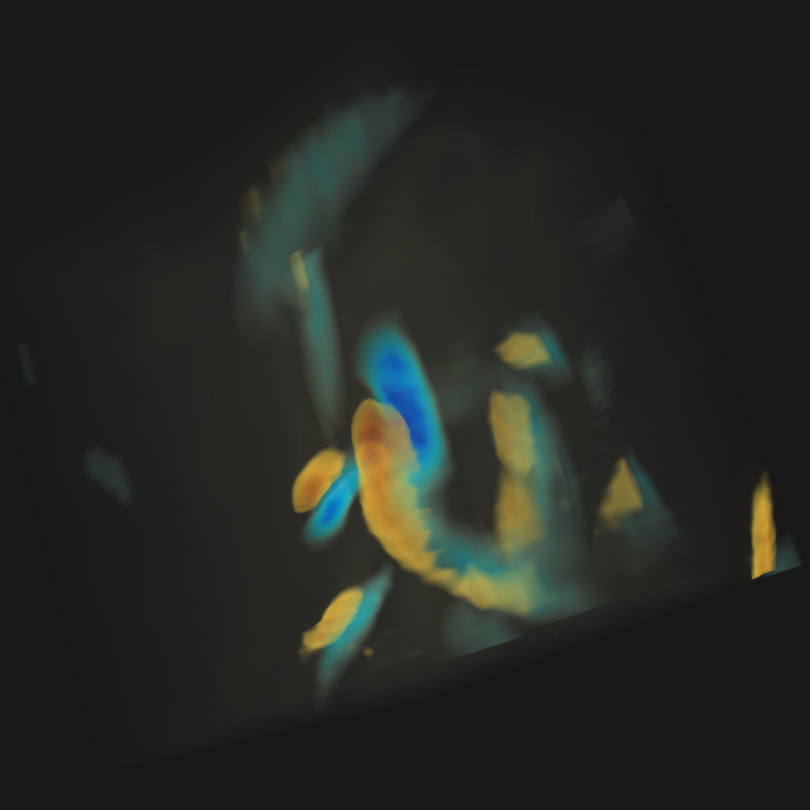
\includegraphics[width=0.16\linewidth]{gradient/gradient-turbulence-wavelet-norm}}}
\subcaptionbox{\emph{by magnitude} (\smag)}{%
{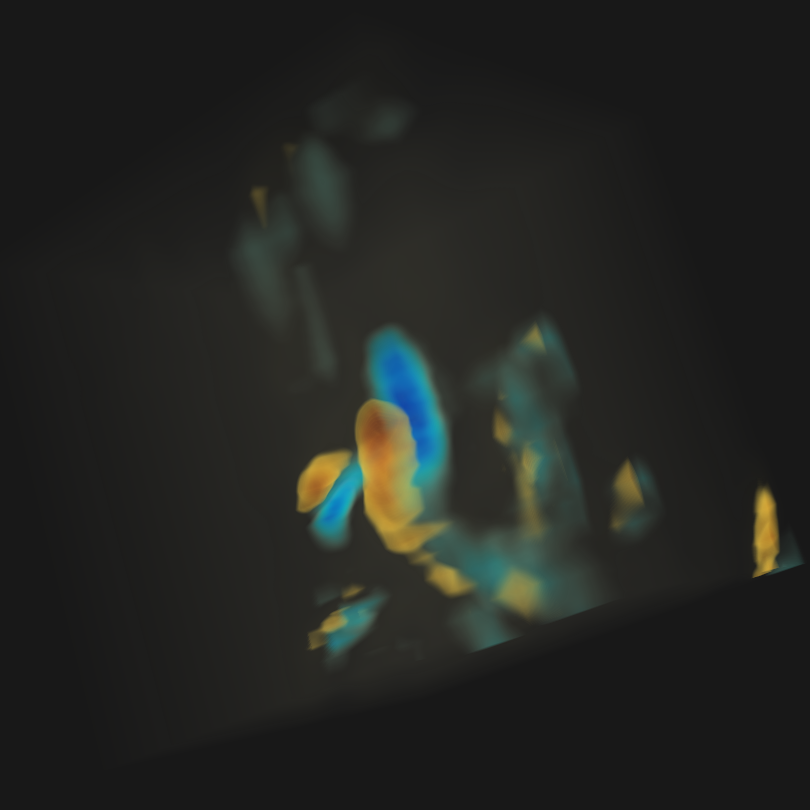
\includegraphics[width=0.16\linewidth]{gradient/gradient-turbulence-magnitude}}}
\subcaptionbox{\emph{by signature} (\sgsg)}{%
{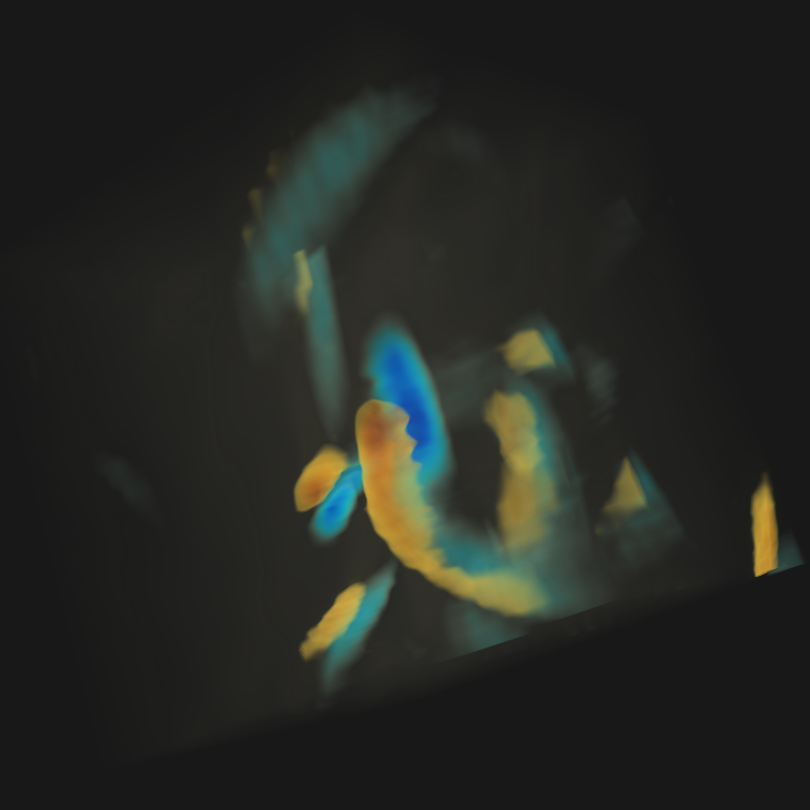
\includegraphics[width=0.16\linewidth]{gradient/gradient-turbulence-signature.png}}}
\subcaptionbox{\emph{ground truth}}{%
{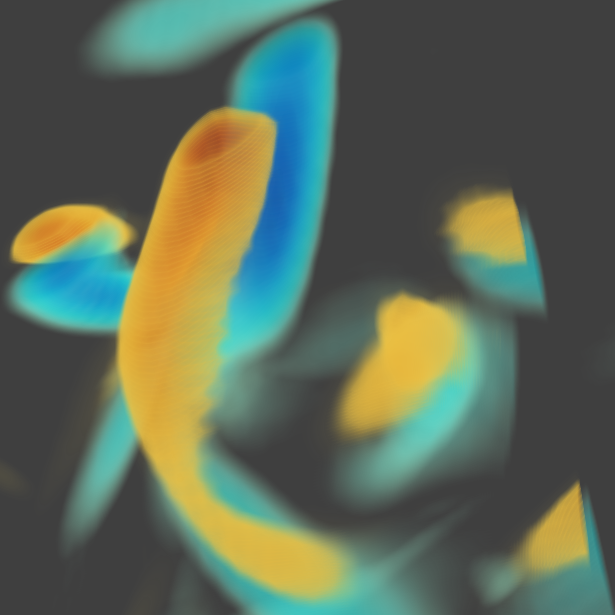
\includegraphics[width=0.16\linewidth]{gradient/gradient-turbulence-groundtruth.png}}}
\caption{$x$-component of the ($64^3$) gradient field of \emph{turbulence}, reconstructed at 0.5
bps. The gradient field produced by \sbit is more accurate than one produced by \swav, and slightly
more accurate than one produced by \sgsg (compare orange features).}
\label{fig:gradient-rendering-diff}
\end{figure*}

\begin{figure}[h]
\centering
\subcaptionbox{\emph{by bit plane} (\sbit)}{
{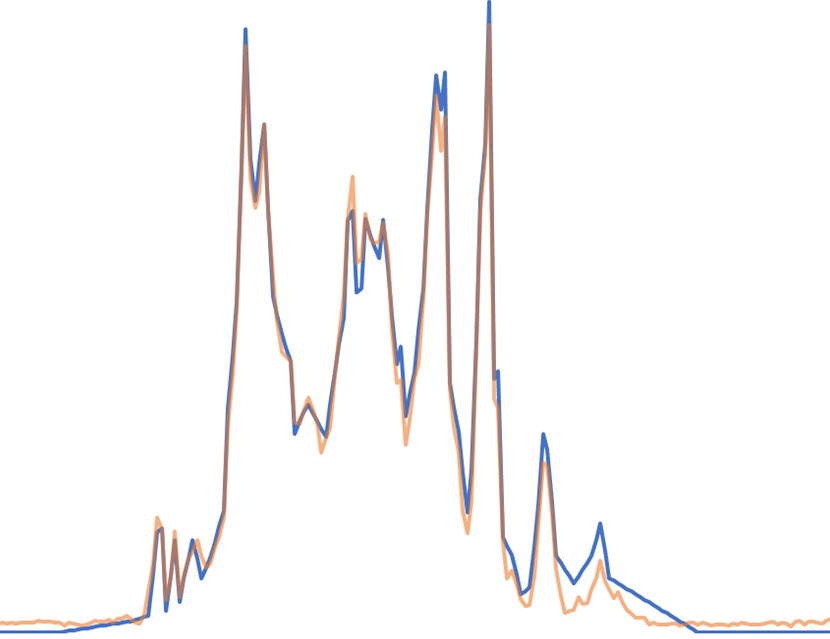
\includegraphics[width=0.48\linewidth]{gradient/gradient-bit-plane}}} 
\subcaptionbox{\emph{by wavelet norm} (\swav)}{
{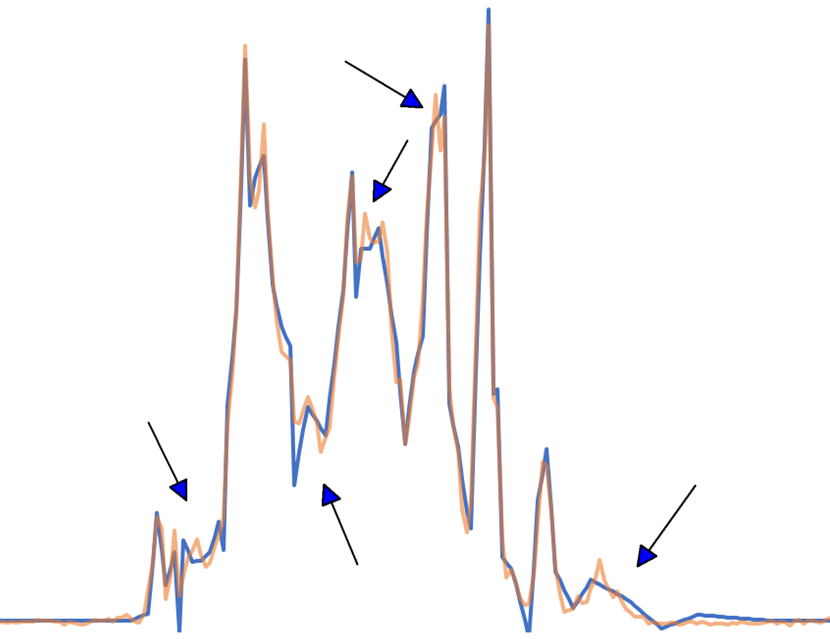
\includegraphics[width=0.48\linewidth]{gradient/gradient-wavelet-norm}}}
\caption{A 1D line extracted from \emph{plasma}, and reconstructed using \sbit and \swav at 0.6 bps.
The original data is in orange and the reconstructions are in blue. \swav captures well the function
values in low-gradient regions, where \sbit struggles (red arrows). However, \sbit retains the shape
of the original function well in areas of both low and high gradients, where \swav instead produces
smooth approximations (blue arrows). \sbit therefore is better for derivative computations, where a
function's shape (or its relative values) matters more than its absolute values.}
\label{fig:bit-plane-vs-wavelet-norm-gradient}
\end{figure}

Given a function $f$ defined on a grid, its gradient at a grid point \mbox{$\x = (x,y,z)$} is the
vector $\nabla f(\x) = \left(\frac{\partial f}{\partial x}, \frac{\partial f}{\partial y},
\frac{\partial f}{\partial z}\right)$. We use a five-point stencil to compute the gradient, i.e.,
$\frac{\partial f}{\partial x} \approx \frac{1}{12}f(x-2,y,z) - \frac{2}{3}f(x-1,y,z) +
\frac{2}{3}f(x+1,y,z) - \frac{1}{12}f(x+2,y,z)$. The error between a gradient field $\nabla f$, and
its low-bit-rate approximation $\nabla
\tilde{f}$, is defined as $\err(\nabla \tilde{f}, \nabla f) = \sqrt{\frac{1}{N}
\sum_{i=1}^{N}{\norm{\nabla \tilde{f}(\x_i)-\nabla f(\x_i)}^2}}$. Using~\Cref{alg:greedy}, we
compute a \emph{gradient-optimized} stream, \sgop, i.e., a stream that minimizes the difference
between the reconstructed gradient field and the original gradient field.

\Cref{fig:gradient-error-comparison} shows the gradient error incurred by different streams for four
data sets. In general, we observe the ordering of performance (from best to worst) as: \sgop, \sgsg,
\sbit, \swav, \smag, \slvl. This ordering can also be seen in~\Cref{fig:gradient-rendering-diff},
where the $x$-component of the gradient field for \emph{tuburlence} is rendered at 0.5 bps. Unlike
the RMSE case, \sbit produces better approximations of the gradient field compared to \swav.

We further investigate this difference by extracting a 1D line from the \emph{plasma} data set and
reconstructing the function using \sbit and \swav at 0.6 bps
(\Cref{fig:bit-plane-vs-wavelet-norm-gradient}). Because the coarse-scale coefficients in \sbit are
approximated at low precision, the reconstruction from \sbit is inaccurate in areas of low
gradients. In contrast, \swav's reconstruction is accurate in low-gradient areas, but lacks the
resolution to resolve the high-gradient areas, because \swav frequently intersperses bits that
improve resolution with bits that improve precision, unlike \sbit, which always streams bits that
improve resolution first. Therefore, \swav tends to produce a ``smoother'' reconstruction that
\emph{on average} (e.g., in terms of RMSE) is close to the original function. \sbit, on the other
hand, tends to capture well the function's shape (due to fine-scale bits), but the whole function
can be ``shifted'' slightly due to the lack of precision in coarse-scale coefficients. However, the
error caused by this shifting reduces significantly when taking the gradient, which cancels any
constant shift. \sbit, therefore, works better than \swav for gradient computation, because it is
better able to retain sharp features.

\sgop again outperforms the rest of the streams. \slvl and \smag perform poorly for gradient
computation, lacking the resolution to capture sharp features. \sgsg closely follows \sbit in
performance (it is slightly better than \sbit for \emph{boiler} at very low bit rates). These
results suggest that while \swav is the best among the data-independent streams when optimizing for
RMSE, \sbit is better for gradient computation.

\subsubsection{Laplacian Computation}\label{sec:laplacian}

\begin{figure*}[h]
\centering
\subcaptionbox{\emph{boiler}}
{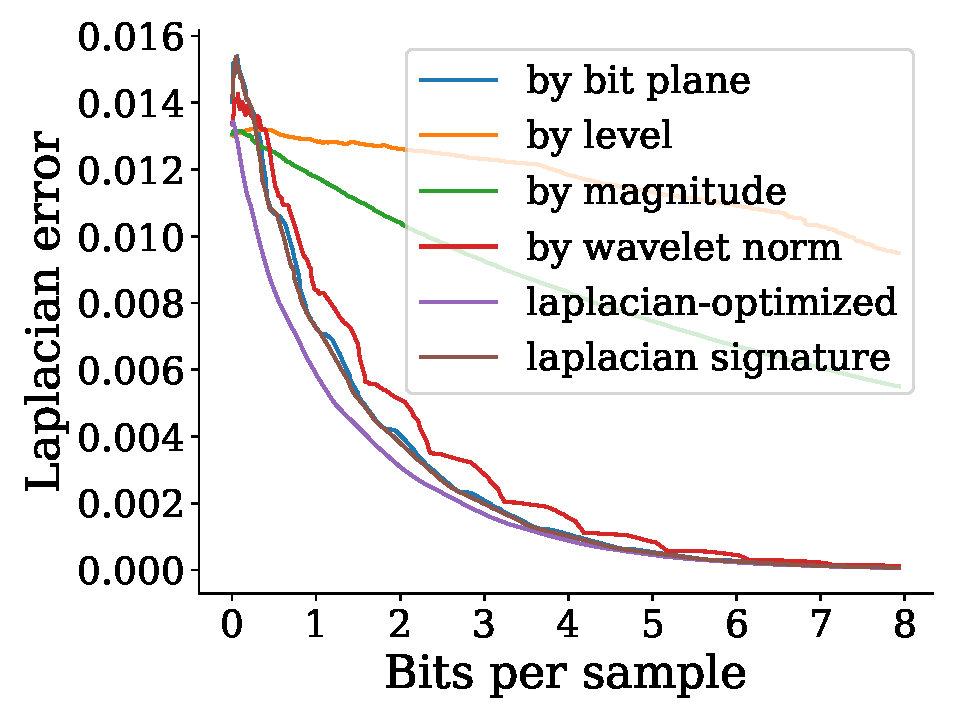
\includegraphics[width=0.24\linewidth]{laplacian/laplacian-optimized-boiler}}
\subcaptionbox{\emph{diffusivity}}
{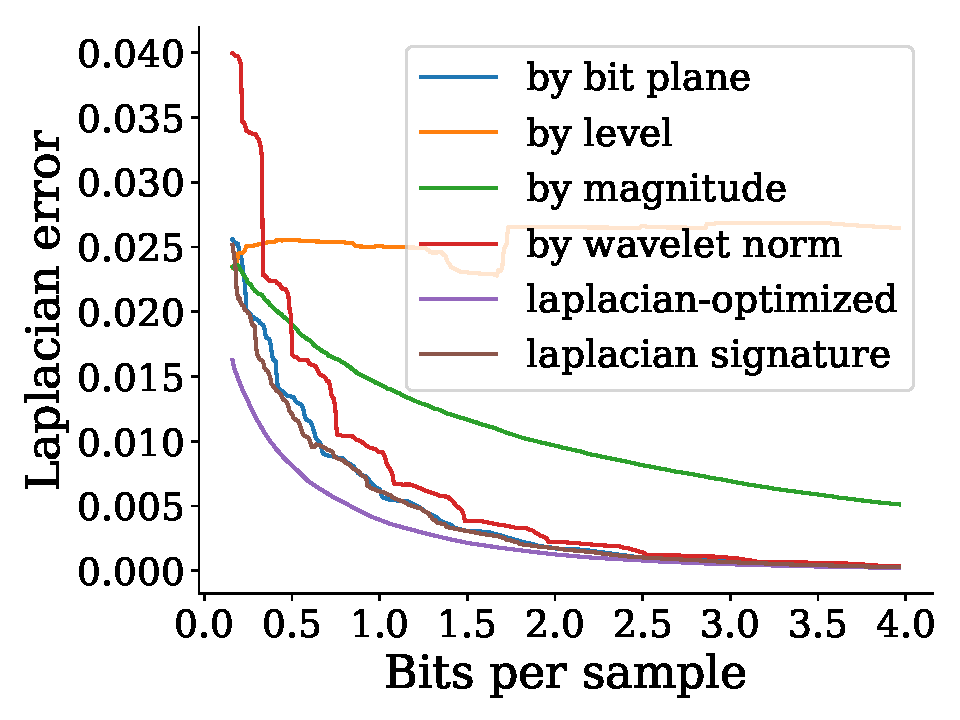
\includegraphics[width=0.24\linewidth]{laplacian/laplacian-optimized-diffusivity}}
\subcaptionbox{\emph{turbulence}}
{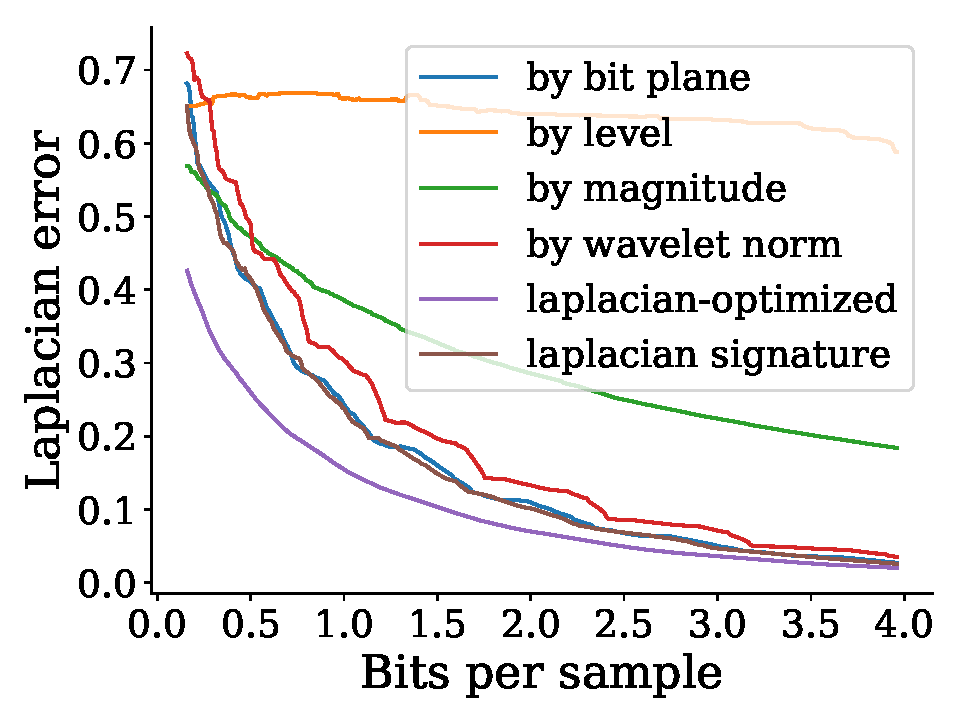
\includegraphics[width=0.24\linewidth]{laplacian/laplacian-optimized-turbulence}}
\subcaptionbox{\emph{pressure}}
{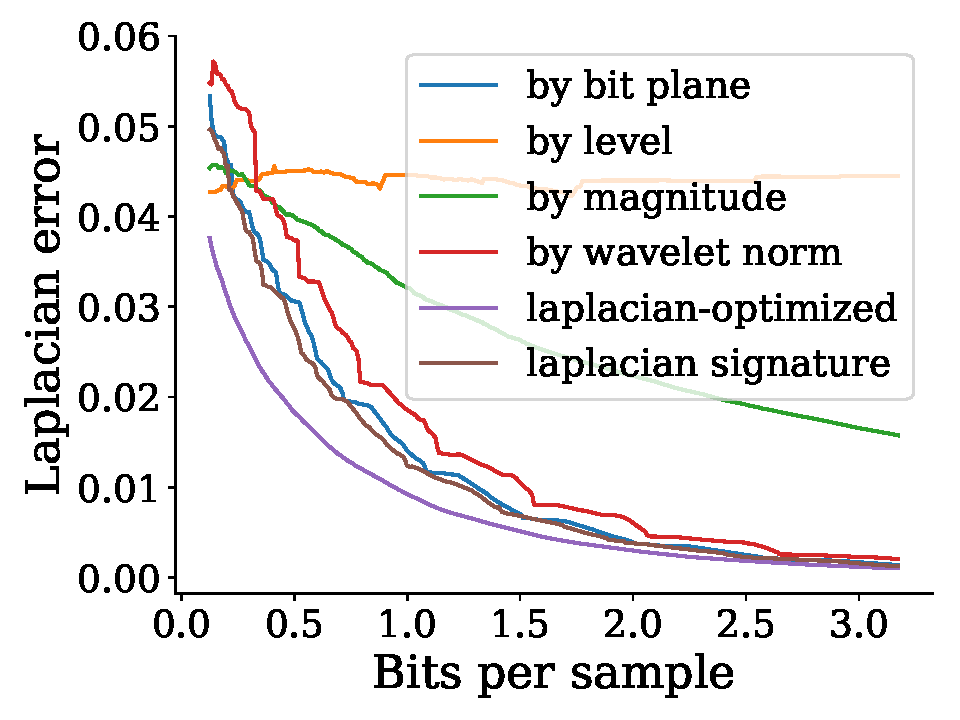
\includegraphics[width=0.24\linewidth]{laplacian/laplacian-optimized-pressure}}
\caption{Laplacian error comparison among streams. The plots are truncated to better highlight
differences without discarding important information. In all cases, in terms of error, $\slop <
\slsg < \sbit < \swav < \smag < \slvl$}.
\label{fig:laplacian-error-comparison}
\vspace{1em}
\end{figure*}

The Laplace operator is a second-order differential operator defined as the divergence of the
gradient field. The Laplacian of a 3D field is defined as $\Delta
f=\frac{{\partial}^2}{\partial{x^2}}f+\frac{{\partial}^2}{\partial{y^2}}f+\frac{{\partial}^2}{\partial{z^2}}f$.

Using a five-point finite difference, we approximate $\frac{{\partial}^2}{\partial{x^2}}f(x,y,z)
\approx
-\frac{1}{12}f(x-2,y,z)+\frac{4}{3}f(x-1,y,z)-\frac{5}{2}f(x,y,z)+\frac{4}{3}f(x+1,y,z)-\frac{1}{12}f(x+2,y,z)$.
We use the root-mean-square error to compare two Laplacian fields, i.e., $\err(\Delta
\tilde{f},\Delta f)=\text{RMSE}(\Delta \tilde{f},\Delta f)$. As usual, we use~\Cref{alg:greedy} to
compute a \emph{Laplacian-optimized} stream, \slop, which minimizes $\err$, and an \slsg stream from
its signature.~\Cref{fig:laplacian-error-comparison} plots the error curves for all relevant
streams. The plots here largely follow the ones in~\Cref{fig:gradient-error-comparison}, in terms of
relative performance among the streams, but with more discernible gaps between \sbit and \slsg.

\subsection{Histogram Computation}\label{sec:histogram}

A histogram succinctly summarizes the distribution of sample values, and thus is useful as a cursory
``look'' into the data and in guiding further analysis. For example, it can be used to guide the
selection of colors and opacities in a transfer function.

To decide on an error metric to compare histograms, we have experimented with several popular
metrics such as Kolmogorov-Smirnov~\cite{smirnov1948}, Kullback-Leibler~\cite{kullback1951}, and
Earth Mover's Distance~\cite{emd1998} among others~\cite{Hellinger1909,Bhattacharyya1943}. We choose
histogram intersection~\cite{histogram_intersection1991} as the metric of choice, because it is fast
to compute and is reasonably insensitive to changes in precision, as well as the number of bins. The
intersection distance between two histograms $H_1$ and $H_2$ is defined as
$\err(H_1,H_2)=1-\sum_{i}{\min{(H_1(i),H_2(i))}}$ (the sum is over all bins $i$). Every histogram is
normalized by dividing the value in each bin by the number of samples in the volume. We have decided
that the error metric should take into account both the histogram shapes and the range of values.
Therefore, we clamp the range of values in reconstructed functions to that of the original function,
so that corresponding histogram bins, i.e., $H_1(i)$ and $H_2(i)$, share the same range. However, in
situations where only the histogram shape but not the range of values is deemed important, no
clamping is needed.

As before, for each data set, we use~\Cref{alg:greedy} to compute an \shop stream, optimized for
histogram error, and then construct an \shsg from its signature. We plot the error curves for all
relevant streams using the Intersection error metric~(compare
\Cref{fig:histogram-stream-comparison}). We use 64 for the number of bins, but note that there exist
no meaningful differences across a wide range of number of bins (from 64 to 512) in our experiments.
In all cases, the group consisting of \sbit, \slvl, and \smag underperforms the other group by a
large margin.

Among the former group of streams, \slvl generally outperforms \sbit at low bit rates, although
there are several crossover points between the two curves~(visualization
in~\Cref{fig:histogram-explain}). When leading zero packets are present, \slvl outperforms \sbit,
because increasing resolution does not help produce an accurate histogram as much as increasing
precision. The histogram is oblivious to spatial locations of samples (which require resolution to
resolve), but is sensitive to sample values (which require precision). However, when leading zero
packets are removed with compression, \sbit benefits significantly more than \slvl does (for the
same reason explained in~\Cref{sec:rmse-optimized}), resulting in the observed crossovers. Finally,
\smag performs poorly, because it ignores regions of smooth variations, which nevertheless count
toward the distribution.

In the latter group, the performances of \swav and \shsg (and even \shop) differ by a negligible
amount. This observation is confirmed in~\Cref{fig:histograms-boiler}, where we plot various
histograms, reconstructed at 0.13 bps, for the \emph{boiler} data set. The histograms produced by
\swav and \shsg have approximately the same shape, and are the closest to the reference histogram.
The next best histogram is produced by \slvl, followed by the one produced by \sbit, and finally
\smag. These results suggest that histogram computation, while being in favor of precision, benefits
significantly from a bit ordering that combines both resolution and precision, not one that adheres
to either exclusively.

\begin{figure*}[t]
	\centering
	\subcaptionbox{\emph{boiler}}
	{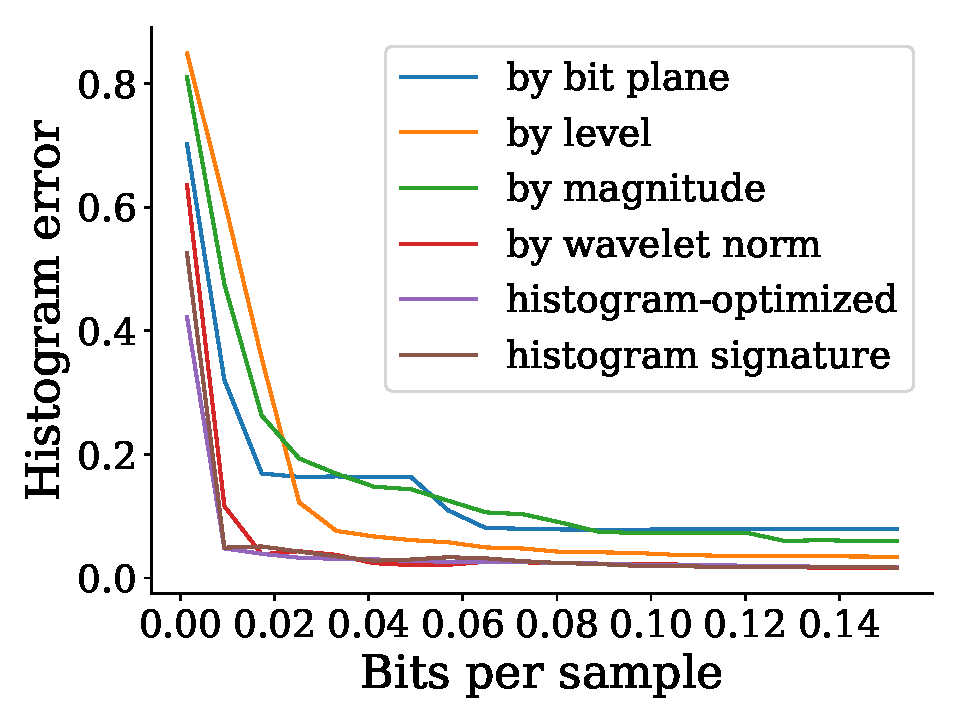
\includegraphics[width=0.24\linewidth]{histogram/histogram-optimized-boiler}}
	\subcaptionbox{\emph{diffusivity}}
	{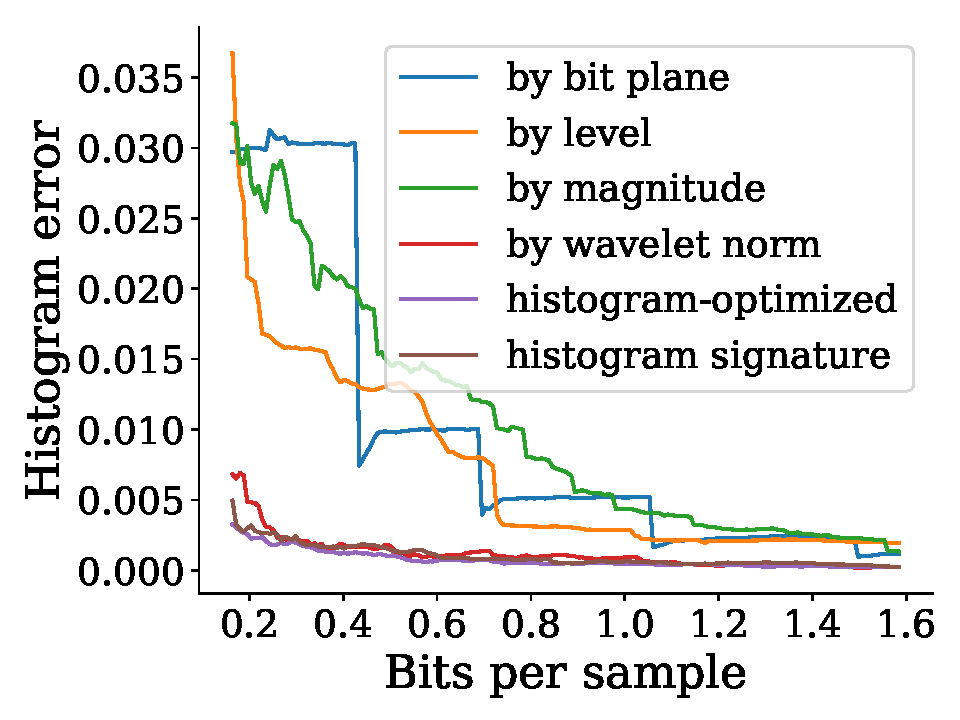
\includegraphics[width=0.24\linewidth]{histogram/histogram-optimized-diffusivity}}
	\subcaptionbox{\emph{kingsnake}}
	{\includegraphics[width=0.24\linewidth]{histogram/histogram-optimized-kingsnake}}
	\subcaptionbox{\emph{foam}}
	{\includegraphics[width=0.24\linewidth]{histogram/histogram-optimized-foam}}
	\caption{Comparison of histogram errors among streams. Plots are truncated to highlight
	differences without hiding important trends. In general, in terms of error, $\shop \approx \shsg
	\approx \swav < \slvl, \sbit, \smag$. The erratic behavior at the beginning for \emph{kingsnake}
	is likely due to the data being too noisy. The especially poor performances of \sbit for
	\emph{boiler} and \emph{foam} are due to the ``shifting'' effect explained in~\Cref{sec:gradient}.
	Crossover points between \sbit and \slvl are explained in~\Cref{fig:histogram-explain}}.
	\label{fig:histogram-stream-comparison}
\vspace{1em}

	\centering
	\subcaptionbox{\emph{by level} (\slvl)}{
	{\includegraphics[width=0.155\linewidth]{histogram/histogram-boiler-level.png}}}
	\subcaptionbox{\emph{by bit plane} (\sbit)}{
	{\includegraphics[width=0.155\linewidth]{histogram/histogram-boiler-bit-plane.png}}}
	\subcaptionbox{\emph{by magnitude} (\smag)}{
	{\includegraphics[width=0.155\linewidth]{histogram/histogram-boiler-magnitude.png}}}
	\subcaptionbox{\emph{by wavelet norm} (\swav)}{
	{\includegraphics[width=0.155\linewidth]{histogram/histogram-boiler-wavelet-norm.png}}}
	\subcaptionbox{\emph{by signature} (\shsg)}{
	{\includegraphics[width=0.155\linewidth]{histogram/histogram-boiler-signature.png}}}
	\subcaptionbox{\emph{reference}}{
	{\includegraphics[width=0.155\linewidth]{histogram/histogram-boiler-groundtruth.png}}}
	\caption{Histograms of the \emph{boiler} data set, reconstructed at 0.13 bps. \slvl, \swav, and
	\shsg produce histograms that share a shape similar to the reference histogram, with most of the
	peaks and valleys preserved. In contrast, \sbit produces a spurious peak not found in the
	reference. Finally, \smag's histogram has a widely skewed distribution where too many values fall
	into the first bin.}
	\label{fig:histograms-boiler}
	\vspace{-1em}
\end{figure*}

\begin{figure*}[t]
\centering
\subcaptionbox{\em pressure, isovalue=0.2}
{\includegraphics[width=0.24\linewidth]{isocontour/isocontour-optimized-pressure}}
\subcaptionbox{\em kingsnake, isovalue=106}
{\includegraphics[width=0.24\linewidth]{isocontour/isocontour-optimized-kingsnake}}
\subcaptionbox{\em plasma, isovalue=2}
{\includegraphics[width=0.24\linewidth]{isocontour/isocontour-optimized-plasma}}
\subcaptionbox{\em turbulence, isovalue=2}
{\includegraphics[width=0.24\linewidth]{isocontour/isocontour-optimized-turbulence}}
\caption{Comparison of isosurface errors among streams. Plots are truncated to highlight differences
without hiding important trends. In all cases, \slvl performs significantly worse than the rest.
\swav outperforms \sbit for \emph{pressure} and \emph{kingsnake}, but not for \emph{plasma} and \emph{turbulence}.}\label{fig:isocontour-plots}
\vspace{1em}

\centering
\subcaptionbox{\emph{by level} ($s_{lvl}$)}
{\includegraphics[width=0.16\linewidth]{isocontour/isocontour-level}}
\subcaptionbox{\emph{by bit plane} ($s_{bit}$)}
{\includegraphics[width=0.16\linewidth]{isocontour/isocontour-bit-plane}}
\subcaptionbox{\emph{by wavelet norm} ($s_{wav}$)}
{\includegraphics[width=0.16\linewidth]{isocontour/isocontour-wavelet-norm}}
\subcaptionbox{\emph{by magnitude} ($s_{mag}$)}
{\includegraphics[width=0.16\linewidth]{isocontour/isocontour-magnitude}}
\subcaptionbox{\emph{by signature} ($s_{iso-sig}$)}
{\includegraphics[width=0.16\linewidth]{isocontour/isocontour-signature}}
\subcaptionbox{\emph{ground truth}}
{\includegraphics[width=0.16\linewidth]{isocontour/isocontour-groundtruth}}
\caption{Rendering of isosurfaces at isovalue of 0.2, at 0.7 bps, for the \emph{pressure} data set.
The surfaces are colored by the $x$-component of the normal vector at each point. \swav and
\sisg produce surfaces that are closest to the reference, followed by \sbit, \smag, and \slvl.}
\label{fig:isocontour-surfaces-pressure}
\end{figure*}

\begin{figure}[h]
	\centering
	\subcaptionbox{with leading zero packets}
	{\includegraphics[width=0.48\linewidth]{histogram/histogram-explain-boiler-wlz}}
	\subcaptionbox{without leading zero packets}
	{\includegraphics[width=0.48\linewidth]{histogram/histogram-explain-boiler}} \caption{Histogram
	error curves produced by \sbit and \slvl, for \emph{boiler}, with and without leading zero bits.
	The vertical axis is in log scale. The error for \sbit reduces in a stair-step fashion, whhere
	each step corresponds to a new bit plane streamed. \sbit benefits significantly more from the
	removal of leading zero bits (the blue curve shifts more to the left).}
	\label{fig:histogram-explain}
	\vspace{-1em}
\end{figure}

\subsection{Isosurface extraction\pavol{update plot text to isosurface}}
\label{sec:isocontour}
Another common visualization task is display of boundaries, usually done using isosurfaces. For example,
isosurface of OH concentration can separate burning and extinguished regions in a combustion simulation or
organs can be extracted from medical imaging by threshold on a CT scalars. Moreover, topological methods such as Reeb Graph is
defined by contracting isosurfaces to a point and building the structure from equivalence classes of isosurfaces.
Extraction of isosurfaces is therefore an essential task in any
visualization and analysis system. We thus study the characteristics of bit streams that
minimize errors in the reconstructed isosurfaces and compare those streams quantitatively and qualitatively.

\pavol{potentially weak point as we do not use any standard error metric here; is the relative surface area fudge
necessary for higher resolution datasets?}
As before, we begin by defining an error metric to compare isosurfaces. Commonly used metric is a Hausdorff
distance that measures the shortest path from a point on one surface to the other, and then taking maximum
of all those paths. Unfortunately, the distance is not very robust and can vary drastically with minor changes
in the surfaces. For example, a single perturbation in one of the two surfaces
can result in a large distance even when the surfaces are close to identical. Therefore, we use a number of
misclassified voxels as our distance which can be computed by counting all voxels that are either in surface $S_1$
and not surface $S_2$ or the other way. \pavol{not sure if following is needed}We have found that if the error caused by
switching off a chunk is too small (in orders of sub-pixel/sub-voxel), then the importance of the
chunk cannot be properly measured. We therefore amend the error metric by adding to it the relative
difference in area between two isosurfaces. This relative difference is, most of the time, a number
between $0$ and $1$, computed by the formula $|A(S_1)-A(S_2)|/A(S_1)$, where $A(S)$ is the area of
an isosurface $S$. The idea is that when the number number of misclassified voxels is less than $1$, the
error -- which is at the sub-voxel level -- is captured by the relative difference in contour length
instead.

With an error metric defined, we can compute an \emph{isosurface-optimized} stream for each data set in addition
to the other streams that are data independent (\Cref{fig:isocontour-plots}). The hypothesis is resolving an
isosurface is primarily affected by the domain resolution.
Both resolution and precision streams are bounded by Nquist limit, a fine isosurface detail may fail
to be resolved either due low resolution or precision. As expected, the {\em isosurface-optimize} stream performs
the best as it has the most freedom when reordering chunks. We observed close to no difference between {\em by bit
plane}, {\em by wavelet norm}, and {\em isosurface signature} streams. This result is primarily caused by the need for
resolution when extracting isosurfaces. For example, {\em by bit plane} stream will always load full resolution data and
vary only precision.

\begin{figure}
	\centering
	\subcaptionbox{pressure}
	{\includegraphics[width=0.48\linewidth]{isocontour/isocontour-optimized-pressure}}
	\subcaptionbox{turbulence}
	{\includegraphics[width=0.48\linewidth]{isocontour/isocontour-optimized-turbulence}}
	\subcaptionbox{plasma}
	{\includegraphics[width=0.48\linewidth]{isocontour/isocontour-optimized-plasma}}
	\subcaptionbox{diffusivity}
	{\includegraphics[width=0.48\linewidth]{isocontour/isocontour-optimized-diffusivity}}
	\caption{Isosurface errors for data-independent, \emph{isosurface-optimized}, and
                 {\em isosurface signature} streams. The bit rates are capped to highlight differences
                 among streams. The {\em by level} and {\em by magnitude} streams performs worst and the other remaining
                 streams have similar performance.}
	\label{fig:isocontour-plots}
\end{figure}

Qualitatively, we studied isosurfaces at specific bit rates for all streams. We were especially interested
at bit rates where the error is not exponentially decaying - the low bit rate isosurfaces do not resemble
the reference full data set isosurfaces. For example, at bit rate 0.4 the error curves are mostly flat and the gaps between
them result in isosurfaces with visible differences (\Cref{fig:isocontour-surfaces})).

\begin{figure}[h]
	\centering
	\subcaptionbox{\emph{by level}}
	{\includegraphics[width=0.31\linewidth]{isocontour/isocontour-pressure-level}}
	\subcaptionbox{\emph{by bit plane}}
	{\includegraphics[width=0.31\linewidth]{isocontour/isocontour-pressure-bit-plane}}
	\subcaptionbox{\emph{by wavelet norm}}
	{\includegraphics[width=0.31\linewidth]{isocontour/isocontour-pressure-wavelet-norm}}
	\subcaptionbox{\emph{by magnitude}}
	{\includegraphics[width=0.31\linewidth]{isocontour/isocontour-pressure-magnitude}}
	\subcaptionbox{\emph{groundtruth}}
	{\includegraphics[width=0.31\linewidth]{isocontour/isocontour-pressure-groundtruth}}
	\caption{Miranda pressure field isosurfaces at bitrate of 0.4 bps.\pavol{what isovalue?} Both {\em by level}
        and {\em by magnitude} stream exhibit severe blocking artifacts compared to the groundtruth. The other streams
        still show smear artifacts, but the overall structure of the isosurfaces is more round and closer to the
        reference.}
	\label{fig:isocontour-surfaces}
\end{figure}

\begin{figure}[h]
	\centering
	\subcaptionbox{\emph{reference}}
	{\includegraphics[width=0.31\linewidth]{isocontour/isocontour2-groundtruth}}
	\subcaptionbox{\emph{by bit plane}}
	{\includegraphics[width=0.31\linewidth]{isocontour/isocontour2-bit-plane}}
	\subcaptionbox{\emph{by wavelet norm}}
	{\includegraphics[width=0.31\linewidth]{isocontour/isocontour2-wavelet-norm}}
	\caption{Miranda pressure field isosurfaces at bitrate of 0.4 bps.\pavol{what isovalue?} Both {\em by level}
        and {\em by magnitude} stream exhibit severe blocking artifacts compared to the groundtruth. The other streams
        still show smear artifacts, but the overall structure of the isosurfaces is more round and closer to the
        reference.}
	\label{fig:isocontour-surfaces}
\end{figure}
%Figure 5: We show that the hybrid and isocontour can diverge somewhat for low-gradient contour.
%Valerio suggested here we coudl also build a "ramp" dataset at different angles and see if the two
%diverges more as the ramp become flatter.

%We argue that if the gradient is low, some noise bits at the end will make an impact, the isocontour
%is very sensitive to noise, and is in general not interesting or meaninfgul to extract.


In this section, we looked at isosurface results for all six streams. The {\em by level} and {\em by magnitude} streams
show blocking artifacts compared to the less severe smearing of {\em by wavelet norm} and {\em by precisio} streams. Therefore,
it seems that one of those latter streams combined with a spatial adaptivity would perform well when isosurface
extraction is desired.

\section{3D Results}
In previous sections, we showed that changing the streaming order can significantly reduce error at given position
in the stream. For example, adaptive RMSE optimized stream outperforms any fixed ordering stream, such as by level,
by bitplane, or by wavelet norm. Moreover, we performed an extensive study on various 2D datasets which shows that
data-dependent stream order offers best results.

However, all experiments were done on mostly on 2D slices of 3D data, since those can be inspected manually in our
tool (\pavol{REF}) and the stream and error computation takes orders of magnitude less time. To validate the results
apply to 3D data, we run the same experiments on the full 3D data sets. Since, the data sets are much larger, we had
to for practical reasons increase the group size from $4^2$ to $16^3$.

We start with reproducing the experiment comparing streaming the data \emph{by level}, \emph{by bit plane},
and \emph{by wavelet norm} (\Cref{fig:motivation-3d-rmse}). In 2D experiments, all data set exhibited the by level
being the worst order, then by bit plane, and the best was by wavelet norm (REF). The 3D results are different as
the by level an by bit plane orders cross. \pavol{WHY?, especially boiler does not have almost any empty space}

\begin{figure}
  \centering
	\subcaptionbox{Boiler}
  {\includegraphics[width=0.48\linewidth]{img/motivation-3d/rmse-boiler.pdf}}
	\subcaptionbox{Diffusivity}
 	{\includegraphics[width=0.48\linewidth]{img/motivation-3d/rmse-diffusivity.pdf}}
	\subcaptionbox{Turbulence}
 	{\includegraphics[width=0.48\linewidth]{img/motivation-3d/rmse-turbulence.pdf}}
	\subcaptionbox{Velocity-z}
 	{\includegraphics[width=0.48\linewidth]{img/motivation-3d/rmse-velocityz.pdf}}
 	\caption{Root-mean-square error of reconstructed functions using the three data-agnostic streams
 	defined in Section \ref{sec:motivation}. Lower is better. The streams are truncated to highlight
 	the differences, without omitting important information. \emph{by wavelet norm} performs best,
 	followed closely by \emph{by bit plane}. We left out \emph{euler} (2D) and \emph{plasma} (buggy) datasets.}
 	\label{fig:motivation-3d-rmse}
\end{figure}



\section{Conclusion}

We presented a study of tradeoff between resolution and precision for commonly used derived
scientific quantities such as RMSE, gradient, Laplacian, histogram, and isosurface.
During this study, we covered the gamut of scientific data sets, ranging from simulations
with smooth features or fine scale detail to image data with noisy parts\pavol{do we have plot of image data?}.
We showed that one stream type does not fit all analysis tasks, but some streams perform well
in most of them and may be useful in a new file format design.

We started with an evaluation of contemporary techniques for reducing resolution or precision.
The experiments showed that streaming only in resolution or precision is suboptimal for all
tested queries. We thus developed a tractable greedy algorithm for computing adaptive stream order
based on the particular task. The produced stream significantly\pavol{it would be good to quantify what
significantly means, 2x?} outperforms any stream that has
a fixed streaming order.

After establishing the greedy algorithm for computing a stream, we focused on each query and
investigated which queries have similar streams. This approach is important because if two streams
are very similar, we can precompute the stream order and apply the same ordering to different
queries.

For example, we learned that the RMSE stream is akin to the gradient stream, and thus only one
needs to be computed. Moreover, since RMSE optimizes for the function, the stream alongside
a good gradient approaches the function itself. In contrast, the gradient ignores the constant offest
of all samples, resulting in an inferior RMSE.


These results should be considered when designing a file format for scientic data. As future work,
we plan to create new file format that will incorporate the stream-ordering techniques we presented.
Additionally, such file format needs to support compression and spatial adaptivity to handle large-scale
data and fast queries. We are investigating if signatures can be used to handle
the spatial adaptivity. For example, we could extend the signature matrix to the tensor, with
the spatial index being the third dimension.




%% if specified like this the section will be committed in review mode
\acknowledgments{
The authors wish to thank A, B, and C. This work was supported in part by
a grant from XYZ (\# 12345-67890).}

%\bibliographystyle{abbrv}
\bibliographystyle{abbrv-doi}
%\bibliographystyle{abbrv-doi-narrow}
%\bibliographystyle{abbrv-doi-hyperref}
%\bibliographystyle{abbrv-doi-hyperref-narrow}

\bibliography{egbibsample}
\end{document}

